\documentclass[a4paper,12pt]{article}

\usepackage{color}
\usepackage{amsmath}
\usepackage{amsthm}
\usepackage{amssymb}
\usepackage{stmaryrd}
\usepackage{mathrsfs,cmll}
\usepackage[sans]{dsfont}
\usepackage{graphicx}

\usepackage{lingmacros} % linguistic macros for enumerating sentences
\usepackage{bussproofs} 
\EnableBpAbbreviations

% Dynamic connectives and quantifiers

\newcommand{\dynexists}{\mathord{\reflectbox{$\mathds{E}$}}}

\newcommand{\dynall}{\mathord{%
\raisebox{\depth}{\rotatebox{180}{$\mathds{A}$}}}}

\newcommand{\dynor}{\mathbin{\mathds{V}}}

\newcommand{\dynand}{\mathbin{%
\reflectbox{\raisebox{\depth}{\rotatebox{180}{${\dynor}$}}}}}

\newcommand{\dynimplies}{\mathbin{%
\mbox{\raisebox{.28ex}{\rule{1.7ex}{.15ex}}%
\hspace{-1.7ex}\raisebox{.73ex}{\rule{1.7ex}{.15ex}}%
\hspace{-.4ex}\raisebox{-.01ex}{\rotatebox{45}{\rule{.83ex}{.15ex}}}%
\hspace{-.69ex}\raisebox{.58ex}{\rotatebox{135}{\rule{.83ex}{.15ex}}}}
}}

\newcommand{\dynneg}{\mathop{%
\mbox{\raisebox{.68ex}{\rule{1.2ex}{.15ex}}%
\hspace{-.15ex}\raisebox{.2ex}{\rule{.15ex}{.63ex}}%
\hspace{.25ex}\raisebox{.2ex}{\rule{.15ex}{.63ex}}\hspace{.15ex}}
}}

%%%%% lambda-terms

\newif\ifatomic
\newif\ifoperator
\newif\ifconj
\newif\ifdisj
\newif\ifdconj
\newif\ifddisj

\def\reset{\atomicfalse\operatorfalse\conjfalse\disjfalse\dconjfalse\ddisjfalse}

% abstraction

\def\abs#1#2%
{\ifatomic%
(\lambda #1 . \, \reset #2)%
\else%
\lambda #1 . \, \reset #2%
\fi\reset}

% application

\def\app#1#2%
{\ifoperator%
\reset\atomictrue\operatortrue #1 \, \reset\atomictrue #2%
\else%
\ifatomic%
(\reset\atomictrue\operatortrue #1 \, \reset\atomictrue #2)%
\else%
\reset\atomictrue\operatortrue #1 \, \reset\atomictrue #2%
\fi%
\fi\reset}

% universal quantification

\def\uquant#1#2%
{\ifatomic%
(\forall #1 . \, \reset #2)%
\else%
\forall #1 . \, \reset #2%
\fi\reset}

% existential quantification

\def\equant#1#2%
{\ifatomic%
(\exists #1 . \, \reset #2)%
\else%
\exists #1 . \, \reset #2%
\fi\reset}

% implication

\def\imp#1#2%
{\ifatomic%
(\reset\atomictrue #1 \rightarrow \reset\atomictrue #2)%
\else%
\reset\atomictrue #1 \rightarrow \reset\atomictrue #2%
\fi\reset}

% conjunction

\def\conj#1#2%
{\ifconj%
\reset\atomictrue\conjtrue #1 \wedge \reset\atomictrue\conjtrue #2%
\else%
\ifatomic%
(\reset\atomictrue\conjtrue #1 \wedge \reset\atomictrue\conjtrue #2)%
\else%
\reset\atomictrue\conjtrue #1 \wedge \reset\atomictrue\conjtrue #2%
\fi%
\fi\reset}

% disjunction

\def\disj#1#2%
{\ifdisj%
\reset\atomictrue\disjtrue #1 \vee \reset\atomictrue\disjtrue #2%
\else%
\ifatomic%
(\reset\atomictrue\disjtrue #1 \vee \reset\atomictrue\disjtrue #2)%
\else%
\reset\atomictrue\disjtrue #1 \vee \reset\atomictrue\disjtrue #2%
\fi%
\fi\reset}

% negation

\def\nega#1%
{\neg \reset\atomictrue #1\reset}

% dynamic universal quantification

\def\duquant#1#2%
{\ifatomic%
(\dynall #1 . \, \reset #2)%
\else%
\dynall #1 . \, \reset #2%
\fi\reset}

% dynamic existential quantification

\def\dequant#1#2%
{\ifatomic%
(\dynexists #1 . \, \reset #2)%
\else%
\dynexists #1 . \, \reset #2%
\fi\reset}

% dynamic implication

\def\dimp#1#2%
{\ifatomic%
(\reset\atomictrue #1 \dynimplies \reset\atomictrue #2)%
\else%
\reset\atomictrue #1 \dynimplies \reset\atomictrue #2%
\fi\reset}

% dynamic conjunction

\def\dconj#1#2%
{\ifdconj%
\reset\atomictrue\dconjtrue #1 \dynand \reset\atomictrue\dconjtrue #2%
\else%
\ifatomic%
(\reset\atomictrue\dconjtrue #1 \dynand \reset\atomictrue\dconjtrue #2)%
\else%
\reset\atomictrue\dconjtrue #1 \dynand \reset\atomictrue\dconjtrue #2%
\fi%
\fi\reset}

% dynamic disjunction

\def\ddisj#1#2%
{\ifddisj%
\reset\atomictrue\ddisjtrue #1 \dynor \reset\atomictrue\ddisjtrue #2%
\else%
\ifatomic%
(\reset\atomictrue\ddisjtrue #1 \dynor \reset\atomictrue\ddisjtrue #2)%
\else%
\reset\atomictrue\ddisjtrue #1 \dynor \reset\atomictrue\ddisjtrue #2%
\fi%
\fi\reset}

% dynamic negation

\def\dnega#1%
{\dynneg \reset\atomictrue #1\reset}

%%%%%%%%%%%%%%%%%%%%%%%%


%------------------------------------------------------------------------------------
\newcommand{\existsA}{\exists}
\newcommand{\existsB}{\dynexists} 

\newcommand{\forallA}{\exists}
\newcommand{\forallB}{\dynall}  

\newcommand{\impA}{\rightarrow}
\newcommand{\impB}{\dynimplies}

\newcommand{\negA}{\neg}
\newcommand{\negB}{\dynneg}

\newcommand{\landA}{\land}
\newcommand{\landB}{\dynand}

\newcommand{\lorA}{\lor}
\newcommand{\lorB}{\dynor} 


%------------------------------------------------------------------------------------
% New Commands: Miscelaneous abbreviations
%------------------------------------------------------------------------------------

\newcommand{\I}[1]{[\![#1]\!]}  % interpretation

\newcommand{\txt}[1]{\textit{#1}} % italic
\newcommand{\defeq}{\doteq} % equal by definition
\newcommand{\logeq}{\equiv} % logical equivalence
\newcommand{\seq}{=_s} % syntactic equality
\newcommand{\nseq}{\neq_s} % syntactic non-equality

\newcommand{\congr}{=_{\alpha}} % alpha-congruent
\newcommand{\ncongr}{\neq_{\alpha}} % alpha non-congruent



\newcommand{\trr}[1]{#1} % this one does not do anything

\newcommand{\Types}{\text{T}} % Types


\newcommand{\upii}[2]{#1 ::  #2}  % list constructor
\newcommand{\sel}{\mathsf{sel} } % selection function
\newcommand{\updt}{\mathsf{upd}}  % discourse update
\newcommand{\D}{\mathbf{D}} % discourse
\renewcommand{\S}{\mathbf{S}} % sentence

\newcommand{\tr}[1]{\overline{#1}} % dynamizing
\newcommand{\ttr}[1]{ \overline{#1}^*} 
\newcommand{\etr}[1]{ \widetilde{#1}} % non-conventional dynamic term

%------------------------------------------------------------------------------------
% New Commands: Lambda Calculus
%------------------------------------------------------------------------------------
\newcommand{\bconv}{\rightarrow_\beta}  %one-step beta reduction
\newcommand{\bred}{\rightarrow^{*}_\beta} %beta reduction
\newcommand{\econv}{\rightarrow_\eta} %eta conversion 


%------------------------------------------------------------------------------------
% New Commands: 
% Abbreviations for distinguishing variables for static and dynamic cases.
% E.g.: \x1 - static, \x2 - dynamic
%------------------------------------------------------------------------------------
\newcommand{\A}[1]{\ifcase #1 \or \AAA\or\AB\or\AC\fi}
\newcommand{\B}[1]{\ifcase #1 \or \BA\or\BB\or\BC\fi}
\newcommand{\R}[1]{\ifcase #1 \or \RA\or\RB\or\RC\fi}
\newcommand{\Q}[1]{\ifcase #1 \or \QA\or\QB\or\QC\fi}
\renewcommand{\P}[1]{\ifcase #1 \or \PA\or\PB\or\PC\fi}
\newcommand{\X}[1]{\ifcase #1 \or \XA\or\XB\or\XC\fi}
\newcommand{\Y}[1]{\ifcase #1 \or \YA\or\YB\or\YC\fi}
\newcommand{\x}[1]{\ifcase #1 \or \xA\or\xB\or\xC\fi}
\newcommand{\y}[1]{\ifcase #1 \or \yA\or\yB\or\yC\fi}
\newcommand{\z}[1]{\ifcase #1 \or \zA\or\zB\or\zC\fi}
\renewcommand{\t}[1]{\ifcase #1 \or \tA\or\tB\or\tC\fi}
\newcommand{\h}[1]{\ifcase #1 \or \hA\or\hB\or\hC\fi}
\renewcommand{\v}[1]{\ifcase #1 \or \vA\or\vB\or\vC\fi}
\renewcommand{\u}[1]{\ifcase #1 \or \uA\or\uB\or\uC\fi}
\newcommand{\w}[1]{\ifcase #1 \or \wA\or\wB\or\wC\fi}

%------------------------------------------------------------------------------------

\newcommand{\AAA}{\mathrm{A}}
\newcommand{\AB}{\mathbf{A}}
\newcommand{\AC}{\varmathbb{A}}

\newcommand{\BA}{\mathrm{B}}
\newcommand{\BB}{\mathbf{B}}
\newcommand{\BC}{\varmathbb{B}}


\newcommand{\RA}{\mathrm{R}}
\newcommand{\RB}{\mathbf{R}}
\newcommand{\RC}{\varmathbb{R}}

\newcommand{\QA}{\mathrm{Q}}
\newcommand{\QB}{\mathbf{Q}}
\newcommand{\QC}{\varmathbb{Q}}

\newcommand{\PA}{\mathrm{P}}
\newcommand{\PB}{\mathbf{P}}
\newcommand{\PC}{\varmathbb{P}}

\newcommand{\XA}{\mathrm{X}}
\newcommand{\XB}{\mathbf{X}}
\newcommand{\XC}{\varmathbb{X}}

\newcommand{\YA}{\mathrm{Y}}
\newcommand{\YB}{\mathbf{Y}}
\newcommand{\YC}{\varmathbb{Y}}

\newcommand{\xA}{x}
\newcommand{\xB}{\mathbf{x}}
\newcommand{\xC}{\mathbf{x}}

\newcommand{\yA}{y}
\newcommand{\yB}{\mathbf{y}}
\newcommand{\yC}{\mathbf{y}}

\newcommand{\zA}{z}
\newcommand{\zB}{\mathbf{z}}
\newcommand{\zC}{\mathbf{z}}

\newcommand{\tA}{t}
\newcommand{\tB}{\mathbf{t}}
\newcommand{\tC}{\mathbf{t}}

\newcommand{\hA}{h}
\newcommand{\hB}{\mathbf{h}}
\newcommand{\hC}{\mathbf{h}}

\newcommand{\vA}{v}
\newcommand{\vB}{\mathbf{v}}
\newcommand{\vC}{\mathbf{v}}

\newcommand{\uA}{u}
\newcommand{\uB}{\mathbf{u}}
\newcommand{\uC}{\mathbf{u}}

\newcommand{\wA}{w}
\newcommand{\wB}{\mathbf{w}}
\newcommand{\wC}{\mathbf{w}}



%------------------------------------------------------------------------------------
% New Commands: Non-logical constants
%------------------------------------------------------------------------------------

\newcommand{\cfarmer}{\textbf{f} }
\newcommand{\cdonkey}{\textbf{d} }
\newcommand{\cown}{\textbf{o} }
\newcommand{\cbeat}{\textbf{b} }

%------------------------------------------------------------------------------------
% New Commands: Frameworks
%------------------------------------------------------------------------------------

\newcommand{\expn}{\chi}  % exception

\newcommand{\G}{G$_0$} % framework introduced in SALT 2006 paper
\newcommand{\GN}{G} % first order framework
\newcommand{\GL}{GL} % higher order framework
\newcommand{\GLex}{GL$\expn$} % dynamic logic with exceptions

\newcommand{\ex}[1]{\ifcase #1 \or \existsA\or\existsB\or\existsC\fi}
\newcommand{\all}[1]{\ifcase #1 \or \forallA\or\forallB\or\forallC\fi}
%\newcommand{\imp}[1]{\ifcase #1 \or \impA\or\impB\or\impC\fi}
\newcommand{\dsj}[1]{\ifcase #1 \or \lorA\or\lorB\or\lorC\fi}
\newcommand{\n}[1]{\ifcase #1 \or \negA\or\negB\or\negC\fi}
\newcommand{\cnj}[1]{\ifcase #1 \or \landA\or\landB\or\landC\fi}

%------------------------------------------------------------------------------------
% New Commands: Colorful symbols for the comparison with DPL
%------------------------------------------------------------------------------------



\newcommand{\ntodl}{h_G}
%\newcommand{trntog}{$h_g$}

\newcommand{\ntodpl}{h_{\textit{DPL}}}

\newcommand{\dpltos}{s_{DPL}}
\newcommand{\mdpltos}[1]{ ( #1 )_{s_\textit{DPL}}}

\newcommand{\dltos}{\textcolor{red}{s_{G}}}
\newcommand{\mdltos}[1]{ \textcolor{red}{(} #1 \textcolor{red}{)_{s_{G}}}}

\newcommand{\dplstodls}{\textcolor{blue}{\lceil \cdot \rceil_S}}
\newcommand{\mdplstodls}[1]{\textcolor{blue}{\lceil}  #1 \textcolor{blue}{\rceil_S}}

\newcommand{\dplstodpll}{\textcolor{cyan}{t^{\lambda}_\textit{DPL}}}
\newcommand{\mdplstodpll}[1]{\textcolor{cyan}{(} #1 \textcolor{cyan}{ )_{t^{\lambda}_\textit{DPL}}}}

\newcommand{\dpltodl}{\textcolor{cyan}{t^{G}_\textit{DPL}}}
\newcommand{\mdpltodl}[1]{\textcolor{cyan}{(} #1 \textcolor{cyan}{ )_{t^{G}_\textit{DPL}}}}


\newcommand{\dpllstodl}{\textcolor{blue}{\lceil \cdot \rceil_L}}
\newcommand{\mdpllstodl}[1]{\textcolor{blue}{\lceil} #1 \textcolor{blue}{\rceil_L}}

\newcommand{\newDPL}{\textit{DPL}^\lambda_L}

\newcommand{\statesDPL}{\textit{DPL}_{S}}
\newcommand{\statesDL}{\GN_S}

\newcommand{\langDPL}{\textit{DPL}_L}
\newcommand{\langDL}{\GN_L}




\newcommand{\qex}{\qed}
%
%       Italized theorem-like environments
%
\newtheorem{theorem}{Theorem}[section]
\newtheorem{conjecture}[theorem]{Conjecture}
\newtheorem{lemma}[theorem]{Lemma}
\newtheorem{proposition}[theorem]{Proposition}
\newtheorem{corollary}[theorem]{Corollary}
\newtheorem{principle}[theorem]{Principle}
%
%       Non-italized theorem-like environments:
%
\newtheorem{@definition}[theorem]{Definition}
\newenvironment{definition}{\begin{@definition}\upshape}{\end{@definition}}
\newtheorem{@remark}[theorem]{Remark}
\newenvironment{remark}{\begin{@remark}\upshape}{\end{@remark}}
\newtheorem{@notation}[theorem]{Notation}
\newenvironment{notation}{\begin{@notation}\upshape}{\end{@notation}}
\newtheorem{@example}[theorem]{Example}
\newenvironment{example}{\begin{@example}\upshape }{ \qex\end{@example}}
\newtheorem{@convention}[theorem]{Convention}
\newenvironment{convention}{\begin{@convention}\upshape}{\end{@convention}}
\newtheorem{@note}[theorem]{Note}
\newenvironment{note}{\begin{@note}\upshape}{\end{@note}}


\title{The title of the paper}
\author{Philippe de~Groote
\and
Ekaterina Lebedeva}
\date{}

\begin{document}
\maketitle

\begin{abstract}
Xxx xxx
\end{abstract}


\section{Introduction}
\section{Mathematical preliminaries} \label{tex:math_prelim}

\cite{Church:1940:A-formulation-of-the-simple-theory-of-types}


In this section, based on~\cite{Barendregt:1981:The-Lambda-Calculus:-Its-Syntax-and-Semantics},~\cite{Barendregt:1992:Lambda-Calculi-with-Types} and~\cite{HindleySeldin:2008:Lambda-Calculus-and-Combinators-an-Introduction}, the basic definitions and theorems of type-free (\ref{sec:A1}) and simply-typed (\ref{sec:A2}) lambda calculus are presented. 

\section{Type-free Lambda Calculus} \label{sec:A1}

\begin{definition}[$\lambda$-terms] The set of \textbf{$\lambda$-terms} $\Lambda$ constructed from an enumerable set of variables $V = \{ v, v_1 ,v_2, \dots\}$ is defined inductively as follows:
\begin{center}
$
\begin{array}{rcll}
x \in V & \Longrightarrow & x \in \Lambda &\\
M,N \in \Lambda &  \Longrightarrow & (MN) \in \Lambda & \text{(\textbf{application})}\\ 
 x \in V, M \in \Lambda&  \Longrightarrow  & (\lambda x.M) \in \Lambda & \text{(\textbf{abstraction})}
\end{array} 
$
\end{center}
\end{definition}

In the term $ (\lambda x.M)$, called abstraction, the variable $x$ is the \textbf{argument} of the function and $M$ is the \textbf{body} of the function. %The variable $x$ is \textbf{bound} by $\lambda$ in  $ (\lambda x.M)$.

\begin{example} \label{app:ex1} The following are $\lambda$-terms:
\begin{align*}
& x \\
& (x_1x_2) \\
& (\lambda x. (x_1 x_2)) \\
& (\lambda x_1. (x_1 x_2)) \\
& ((\lambda x. (x_1 x_2)) x_3 ) 
\end{align*}
\end{example}


\begin{remark}[Parenthesis conventions] \label{rem:parcon}
\begin{itemize}
\item application is left-associative
$$MN_1 N_2 \dots N_n \seq (\dots ( (MN_1) N_2 ) \dots N_n)$$
\item  a sequence of $\lambda$-abstractions $\lambda x_1. (\lambda x_2. ( \dots (\lambda x_n. M) )  ) $ is abbreviated as \\ $\lambda x_1 x_2 \dots x_n.M$
$$\lambda x_1 x_2 \dots x_n.M \seq \lambda x_1. (\lambda x_2. ( \dots (\lambda x_n. M) )  )  $$
\item parentheses surrounding the body of an abstraction can be dropped
$$\lambda x_1 x_2 \dots x_n.(M) \seq \lambda x_1 x_2 \dots x_n.M$$
\item outermost parentheses can be dropped 
$$(M) \seq M$$
\end{itemize}
\end{remark}
%application has a higher precedence than abstraction. 
Note that according to the conventions on parentheses, term $\lambda x. MN$ is a more concise way of writing $\lambda x. (MN)$ and is not equivalent to $(\lambda x. M)N$. 

\begin{example} According to Remark~\ref{rem:parcon}, the $\lambda$-terms in Example~\ref{app:ex1} can be written as follows:
\begin{align*}
& x \\
& x_1x_2 \\
& \lambda x. x_1 x_2 \\
& \lambda x_1. x_1 x_2 \\
& (\lambda x. x_1 x_2) x_3 
\end{align*}
\end{example}



\begin{definition}[Free and bound variables] A variable $x$ is \textbf{free} in a $\lambda$-term $M$ if $x$ is not in the scope of $\lambda x$. If $x$ is in the scope of $\lambda x$, it is \textbf{bound}.
\end{definition}

\begin{example} In the term $ (\lambda x. x_1 x_2)$, the variables $x_1$ and $x_2$ are free. In the term $(\lambda x_1. x_1 x_2)$, the variable $x_1$ is bound and the variable $x_2$ is free. In the term $x(\lambda x.x)$, the variable occurs free in the subterm $x$ and bound in the subterm $\lambda x.x$. 
\end{example}

\begin{definition}[Closed $\lambda$-terms] \ 
\begin{enumerate}
\item The set of \textbf{free variables} of $M$, $FV(M)$ is defined inductively as follows:
\begin{align*}
 FV(x)  & = \{ x \} \\
 FV(\lambda x.M)  & = FV(M) - \{ x \} \\
 FV(MN)  & = FV(M) \cup FV(N)
\end{align*}
\item M is \textbf{closed} or a \textbf{combinator}, if $FV(M) = \emptyset$
%\item The result of \textbf{substitution} of $N$ for (the free occurrences of) $x$ in $M$, denoted $x[x:=N]$, is defined as follows ($x \neq y$):
%\begin{center}
%$
%\begin{array}{rcl}
%x[x:=N] & \defeq & N \\
%y[x:=N] &  \defeq & y\\ 
%(PQ)[x:=N]&  \defeq  & (P[x:=N])(Q[x:=N])\\
%(\lambda y.P)[x:=N] & \defeq & \lambda y.(P[x:=N]) \\
%(\lambda x.P)[x:=N] & \defeq & \lambda x.P
%\end{array} 
%$
%\end{center}
\end{enumerate}
\end{definition}

If an equation $M=N$ is provable in the lambda calculus, the provability is denoted by $\lambda \vdash M = N$
or sometimes just by $M=N$.

\begin{definition}[Axioms and rules] For all $M,N, L,Z \in \Lambda$ the following axioms and rules hold:
\begin{prooftree}
\AXC{} \RightLabel{$\beta$-conversion}
\UIC{$(\lambda x.M)N = M[x:=N]$}
\end{prooftree}

\begin{prooftree}
\AXC{}
\UIC{$M = M$}
\end{prooftree}

\begin{prooftree}
\AXC{$M = N$}
\UIC{$N = M$}
\end{prooftree}

\begin{prooftree}
\AXC{$M=N$}
\AXC{$N=L$}
\BIC{$M=L$}
\end{prooftree}

\begin{prooftree}
\AXC{$M=N$}
\UIC{$MZ=NZ$}
\end{prooftree}

\begin{prooftree}
\AXC{$M=N$}
\UIC{$ZM=ZN$}
\end{prooftree}

\begin{prooftree}
\AXC{$M=N$} \RightLabel{rule $\xi$}
\UIC{$\lambda x.M=\lambda x.N$}
\end{prooftree}

\end{definition}

Importantly, substitution $[x:=N]$ in $M$, denoted $M[x:=N]$, is only applicable to the free occurrences of $x$ in $M$. For example,
\begin{align*}
(xy(\lambda x.x))[x:=N] = Ny(\lambda x.x)
\end{align*}

\begin{definition}[Substitution] The result of \textbf{substitution} of $N$ for the free occurences of $x$ in $M$, i.e. $M[x:=N]$, is defined inductively on the structure of $M$ as follows:
\begin{align*}
 x[x:=N] \defeq  \ & N \\
 y[x:=N] \defeq  \ &  y \ \ \text{provided} \ x \nseq y \\
 (\lambda y.M_1)[x:=N] \defeq   \ & \lambda y. (M_1 [x:=N]) \\
 (M_1 M_2)[x:=N] \defeq  \  & (M_1[x:=N])(M_2[x:=N]) \\
 (\lambda x.M_1)[x:=N]  \defeq \ & \lambda x.M_1
\end{align*}

\end{definition}

\begin{lemma}[Substitution lemma] If  $x \nseq y$ and $x \notin FV(L)$, then
\begin{align*}
 M[x:=N][y:=L] \seq M[y:=L][x:=N[y:=L]]
\end{align*}
\end{lemma}
\begin{proof} The proof is by induction on the structure of $M$.
\end{proof}


When performing a substitution $M[x:=N]$, it is necessary to rename those bound variables in $M$ that are free in N. Otherwise, the substitution 
may lead to a false result. For example, without renaming the bound variable $x$ in $\lambda x.xy$, the substitution  $(\lambda x.xy)[y:=x]$ leads to the term $\lambda x.xx$ that acts differently from the desired term, because the free variable $x$ became bound. However, changing $x$ to $z$, for example, before making the substitution, leads to the desired term $\lambda z.zx$. 

\begin{definition}[$\alpha$-conversion] A \textbf{change of bound variable} $x$ in $M$, or an \textbf{$\alpha$-conversion} in $M$, is the replacement of an occurrence of $\lambda x.N$ in $M$ by $\lambda y.(N[x:=y])$, where $y$ does not occur in $N$.
\end{definition}

\begin{definition}[$\alpha$-congruency] $M$ and $N$ are \textbf{$\alpha$-congruent}, denoted $M \congr N$, if one can result from the other by a finite series of changes of bound variables.
\end{definition}

\begin{example}
\begin{align*}
& \lambda x.xy \congr \lambda z.zy \ncongr \lambda x.xx \\
& \lambda xy.yx(\lambda x.x) \congr \lambda xy. yx(\lambda z.z)  \congr \lambda zy. yz(\lambda x.x) \\
& \lambda xy.yx\congr  \lambda zy. yz \congr  \lambda zx. xz \congr \lambda yx. xy 
\end{align*}
\end{example}

It is natural to identify the terms that are $\alpha$-congruent, as they represent the same processes. Moreover, the same processes can be represented by different terms. For example, $\lambda x.Mx$ and $M$ both lead to $MN$ when applied to $N$. Hence, the following rule can be introduced:
\begin{definition}[Extensionality] \textbf{Extensionality} is the following derivation rule, provided $x \notin FV(MN)$:
\begin{prooftree}
\AXC{$Mx = Nx$}
\UIC{$M = N$}
\end{prooftree}
\end{definition}
The extensionality rule allows to prove $\lambda x. Mx = M$. Alternatively,  $\lambda x. Mx = M$ can be considered to be an axiom:
\begin{definition}[$\eta$-conversion] Let $x \notin FV(M)$. Then
\begin{prooftree}
\AXC{} \RightLabel{$\eta$-conversion}
\UIC{$\lambda x. Mx = M$}
\end{prooftree}
\end{definition}

\begin{definition}[$\beta$-normal form]
\begin{enumerate}
\item $M$ is a \textbf{$\beta$-normal form}, if $M$ has no subterm of the form $(\lambda x.L)K$
\item $M$ \textbf{has a $\beta$-normal form}, if there exists an $N$ such that $N$ is a $\beta$-normal form and $N = M$.
\end{enumerate}
\end{definition}

When $M$ is a $\beta$-normal form, it is often said that $M$ is in normal form.

\begin{example} \
\begin{enumerate}
\item $\lambda x.x$ is in normal form.
\item $(\lambda x.x)y$ has a normal form, namely $y$.
\item $(\lambda xy.y)z$ has a normal form, namely $(\lambda y.y)$.
\item $(\lambda xy.x)z$ has a normal form, namely $z$.
\item $(\lambda x.xx)(\lambda y.yy)$ has no normal form.
\end{enumerate}
\end{example}

A notion of reduction on $\Lambda$ is a binary relation on $\Lambda$. The classical notion of reduction $\beta$ is defined as follows:
\begin{definition} $\beta = \{ ( (\lambda x. M)N , M[x:=N] ) | M, N \in \Lambda  \} $
\end{definition}

\begin{definition}[$\beta$-redex, $\beta$-contractum] 
A \textbf{$\beta$-redex} is a term $M$ such that $(M,N) \in \beta$ for some term $N$. In this case $N$ is called \textbf{$\beta$-contractum} of $M$.
\end{definition}

\begin{definition} The notion of reduction $\beta$ induces the following binary relations:
\begin{align*}
\bconv \  & \textbf{one-step } \beta \textbf{-reduction} \\
\bred \  &  \beta \textbf{-reduction} \\
=_{\beta} \  & \beta \textbf{-equality} \text{ (also called } \beta \textbf{-convertibility}\text{)} 
\end{align*}
These relations are inductively defined as follows:
\begin{center}
$
\begin{array}{rcl}
(M,N) \in \beta & \Longrightarrow & M \bconv N \\
M \bconv N &  \Longrightarrow & ZM \bconv ZN \\ 
M \bconv N &  \Longrightarrow & MZ \bconv NZ \\ 
M \bconv N & \Longrightarrow & \lambda x.M \bconv \lambda x.N \\
& & \\
M \bconv N &  \Longrightarrow & M \bred N \\ 
M \bred M & \\ 
M \bred N, N \bred Z & \Longrightarrow & M \bred Z \\
&& \\
M \bred N &  \Longrightarrow & M =_{\beta} N \\ 
M =_{\beta} N & \Longrightarrow & N =_{\beta} M\\ 
M =_{\beta} N, N =_{\beta} Z & \Longrightarrow & M =_{\beta} Z 
\end{array} 
$
\end{center}


%\begin{enumerate}
%\item $(M,N) \in \beta$
%\end{enumerate}

\end{definition}

The notions of $\beta$-redex and $\beta$-equality allow to give an alternative, more formal, definition of $\beta$-normal form:
\begin{definition}[$\beta$-normal form]  
\begin{enumerate}
\item A term $N$ is called a $\beta$-normal form, if $N$ does not contain (as subterm) any $\beta$-redex.
\item A term $N$ is a $\beta$-normal form of $M$, if $N$ is a $\beta$-normal form and $M =_{\beta} N$.
\end{enumerate}
\end{definition}

%\begin{definition}[$\beta$-contractum, $\beta$-redex] Any term of the form 
%\begin{align*} (\lambda x.M)N
%\end{align*}
%is called a \textbf{$\beta$-redex} and the corresponding term
%\begin{align*} M[x:=N]
%\end{align*}
%is called its \textbf{contractum}.
%\end{definition}

%
%\begin{definition}[$\beta$-contracting, $\beta$-reducing]ff
%\end{definition}

The notion of $\beta$-reduction is very important, because it characterizes provability in $\lambda$ and it is Church-Rosser:

\begin{proposition} $M =_{\beta} N$ iff $\lambda \vdash M = N$
\end{proposition}
\begin{proof} See~\cite[p.59]{Barendregt:1981:The-Lambda-Calculus:-Its-Syntax-and-Semantics}.
%\begin{itemize}
%\item Assume $\lambda \vdash M = N$. Use the induction on the length of the proof of $M=N$.
%\item Assume $M =_{\beta} N$. Show by induction on the definition of the relations involved that
%\end{itemize}
\end{proof}


\begin{theorem}[Church-Rosser theorem for $\bred$] If $L \bred M$ and $L \bred N$, then there exists a term $Z$ such that $M \bred Z$ and $N \bred Z$.
\end{theorem}
\begin{proof} See~\cite[p.62]{Barendregt:1981:The-Lambda-Calculus:-Its-Syntax-and-Semantics} or~\cite[p.289]{HindleySeldin:2008:Lambda-Calculus-and-Combinators-an-Introduction}.
\end{proof}
\begin{figure}[h!]
  \centering
    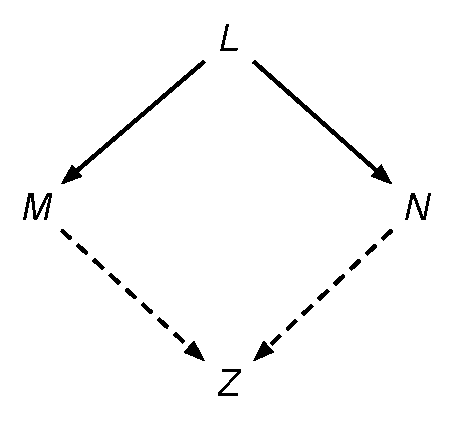
\includegraphics[width=0.3\textwidth]{images/Diamond.pdf}
      \caption{Diamond property.} \label{fig:diamond}
\end{figure}

The Church-Rosser theorem says that for two $\beta$-convertible terms, there is a term to which they both $\beta$-reduce, as illustrated in Figure~\ref{fig:diamond}. The property described in the theorem, that if a term can be reduced to two different terms, then these two terms can be further reduced to one term, is called the \textbf{diamond property} or \textbf{confluence}. The theorem states that $\beta$-reduction is confluent.

\section{Simply-typed Lambda Calculus}  \label{sec:A2}

Lambda terms can be assigned expressions, called ``types'', to denote their intended input and output sets. There exists two typing paradigms: 
\`{a} la Curry, sometimes called \textbf{implicit}, and \`{a} la Church, sometimes called \textbf{explicit}. This section first recalls the basics of Curry-style approach and then briefly compares it with the Church-style.

\begin{definition}[Simple types] Given a set $A$ of \textbf{atomic types}, the set of \textbf{types} $T$ is inductively defined as follows:
\begin{center}
$
\begin{array}{rcll}
\alpha \in A & \Longrightarrow & \alpha \in T &\\
\alpha, \beta \in A &  \Longrightarrow & (\alpha \rightarrow \beta) \in T & \text{(\textbf{function types})}
\end{array} 
$
\end{center}
\end{definition}
An atomic type is intended to denote some particular set. A function type $(\alpha \rightarrow \beta)$ is intended to denote some set of functions from $\alpha$ to $\beta$, i.e. the functions that take as the argument a member of the set denoted by $\alpha$ and return as an output a member of the set denoted by $\beta$.


\begin{remark}[Parenthesis convention] A complex functional type $(\alpha_1 \rightarrow (\alpha_2 \rightarrow \dots \rightarrow (\alpha_{n-1} \rightarrow \alpha_n)  \dots ))$ is abbreviated as $\alpha_1 \rightarrow \alpha_2 \rightarrow \dots \rightarrow \alpha_n$ (i.e. parentheses are associated to the right):
\begin{align*}
(\alpha_1 \rightarrow (\alpha_2 \rightarrow \dots \rightarrow (\alpha_{n-1} \rightarrow \alpha_n)  \dots )) & \seq \alpha_1 \rightarrow \alpha_2 \rightarrow \dots \rightarrow \alpha_n
\end{align*}
\end{remark}


\begin{definition}[$\lambda\!\rightarrow$-Curry]
\begin{enumerate}
\item A \textbf{statement} is of the form $M:\sigma$ with $M \in \Lambda$ and $\sigma \in T$. The type $\sigma$ is the \textbf{predicate} and the term $M$ is the \textbf{subject} of the statement.
\item A \textbf{declaration} is a statement with a variable as a subject.
\item A \textbf{basis} is a set of declarations with distinct variables as subjects.
\end{enumerate}
\end{definition}


\begin{definition}[Derivation rules in $\lambda\!\rightarrow$-Curry] A statement $M:\sigma$ is \textbf{derivable} from a basis $\Gamma$, denoted $\Gamma \vdash_{\lambda\rightarrow \text{-Curry}} M: \sigma$ , $\Gamma \vdash_{\lambda\rightarrow} M: \sigma$ or simply $\Gamma \vdash M: \sigma$, if $\Gamma \vdash M: \sigma$ can be produced by the following rules:
 
\begin{prooftree}
\AXC{} \RightLabel{axiom}
\UIC{$\Gamma, x: \alpha \vdash x: \alpha $}
\end{prooftree} 
 
 \begin{prooftree}
\AXC{$\Gamma \vdash M: \alpha \rightarrow \beta$}
\AXC{$\Gamma \vdash N: \alpha$} \RightLabel{app}
\BIC{$\Gamma \vdash MN: \beta$}
\end{prooftree}

\begin{prooftree}
\AXC{$\Gamma, x: \alpha \vdash M:\beta$} \RightLabel{abs}
\UIC{$\Gamma \vdash \lambda x.M: \alpha \rightarrow \beta$}
\end{prooftree}

\end{definition}


%\begin{definition}
%
%\medskip \noindent \textbf{Compatibility rules}:
%
%\begin{prooftree}
%\AXC{} \RightLabel{if $x$ is a variable}
%\UIC{$x \evalto x$}
%\end{prooftree}
%
%\begin{prooftree}
%\AXC{} \RightLabel{if $c$ is a constant}
%\UIC{$c \evalto c$}
%\end{prooftree}
%
%\begin{prooftree}
%\AXC{$M \evalto N$}
%\UIC{$\lambda x. M \evalto \lambda x.N $}
%\end{prooftree}
%
%\begin{prooftree}
%\AXC{$M \evalto \lambda x. K$}
%\AXC{$Q \evalto N$}
%\AXC{$K[x:=N] \evalto O$}
%\TIC{$ MQ \evalto O$}
%\end{prooftree}
%
%\begin{prooftree}
%\AXC{$M \evalto x$}
%\AXC{$Q \evalto N$}
%\BIC{$ MQ \evalto xN$}
%\end{prooftree}
%
%\begin{prooftree}
%\AXC{$M \evalto OK$}
%\AXC{$Q \evalto N$}
%\BIC{$ MQ \evalto OKN$}
%\end{prooftree}
%\end{definition}

\begin{lemma}[Substitution lemma for $\lambda\!\rightarrow$-Curry] \label{lem:substitution-Curry} \
\begin{enumerate}
\item If $\Gamma \vdash M:\sigma$, then $\Gamma[\alpha :=\tau] \vdash M:\sigma[\alpha :=\tau]$.
\item Suppose $\Gamma, x: \sigma \vdash M: \tau$ and $\Gamma \vdash N: \sigma$. Then $\Gamma \vdash M[x:=N]: \tau$.
\end{enumerate}
\end{lemma}
\begin{proof} 
\begin{enumerate}
\item The proof is by induction on the derivation of $M:\sigma$.
\item The proof is by induction on the generation of $\Gamma, x: \sigma \vdash M:\tau$
\end{enumerate}
\end{proof}

The following theorem states that the set of terms having a certain type is closed under reduction:
\begin{theorem}[Subject reduction theorem for $\lambda\!\rightarrow$-Curry] Suppose $M \bred N$. Then 
\begin{center}
$
\begin{array}{rcl}
\Gamma \vdash M: \sigma &\Longrightarrow & \Gamma \vdash N: \sigma
\end{array}
$
\end{center}
\end{theorem}
\begin{proof} See~\cite[p.41]{Barendregt:1992:Lambda-Calculi-with-Types}.
\end{proof}

While in Curry's approach each term is assigned a type after the term has been built, in Church's approach, the type of a term is integrated in the term itself. For example, the term $\lambda x.x$ can be assigned a type according to the Curry and Church styles respectively as follows:
\begin{align*}
& \vdash_{Curry} \lambda x.x: (\sigma \rightarrow \sigma) \\
& \vdash_{Church} \lambda x^\sigma.x: (\sigma \rightarrow \sigma) 
\end{align*}
The term $\lambda x^\sigma.x$ itself is annotated in a Church system by $\sigma$. This means that $\lambda x^\sigma.x$ takes the argument $x$ from the particular set denoted by $\sigma$. In contrast, a Curry system allows each term to have a polymorphic type. For example, the term $\lambda x.x:  (\sigma \rightarrow \sigma)$ denotes the operation of doing nothing regardless how $\sigma$ is instantiated: it can stand, for example, for integers or for booleans. 

\begin{definition}[$T$-annotated $\lambda$-terms] Let $V$ be a set of variables, $T$ be a set of types. The set $\Lambda_T$ of $T$\textbf{-annotated} $\lambda$\textbf{-terms} is defined as follows:
\begin{center}
$
\begin{array}{rcl}
x \in V & \Longrightarrow & x \in \Lambda_T \\
M, N \in  \Lambda_T& \Longrightarrow & MN \in \Lambda_T \\
x \in V, M \in \Lambda_T, \sigma \in T & \Longrightarrow & \lambda x^\sigma.M \in \Lambda_T
\end{array}
$
\end{center}
\end{definition}

The typed lambda calculus  \`{a} la Church is defined similarly to the typed lambda calculus  \`{a} la Curry: an important difference is in the derivation rule corresponding to the abstraction: the abstracted variable is explicitly annotated with a type in the Church-style system.
The explicit annotation of types in Church-style system makes it possible to decide whether a term has a certain type. This is an undecidable question for some Curry systems. On the other hand, a Curry-style system has more power and more flexibility than a Church-style system. For example, the easiest way to answer the question whether an untyped term $M$ has any typed analogues is to re-state the question in Curry's notation. Furthermore, Curry-style systems can be generalized in ways Church-style systems cannot. 

Terms \`{a} la Church can be easily mapped into terms \`{a} la Curry. This is done simply by ``erasing'' all type annotations within the term \`{a} la Church:
\begin{definition} $| \cdot |: \Lambda_T \rightarrow \Lambda$ is defined as follows:
\begin{center}
$
\begin{array}{rcl}
|x|& \defeq & x \\
|MN|& \defeq & |M||N| \\
|\lambda x^{\sigma}.M|& \defeq & \lambda x.|M|
\end{array}
$
\end{center}
\end{definition}
The following proposition states that terms in the Church version project to terms in the Curry version of $\lambda\!\rightarrow$; and that terms in the Curry style can be ``lifted'' to terms in the Church style:
\begin{proposition}  
\ 
\begin{enumerate}
\item Let $M \in \Lambda_T$. Then
\begin{align*}
\Gamma \vdash_{Church} M:\sigma  \ \ \Longrightarrow \ \ & \Gamma \vdash_{Curry} |M|:\sigma
\end{align*}
\item Let $N\in \Lambda$. Then
\begin{align*}
\Gamma \vdash_{Curry} N:\sigma  \ \  \Longrightarrow \ \ & \text{exists } M  \in \Lambda_T  \\
& \text{such that }  \Gamma \vdash_{Church}  M:\sigma \text{ and } |M| \congr N
\end{align*}
\end{enumerate}
\end{proposition}
\begin{proof} Both (1) and (2) are proved by induction on the given derivation.
\end{proof}
See~\cite{Barendregt:1992:Lambda-Calculi-with-Types}  and~\cite{HindleySeldin:2008:Lambda-Calculus-and-Combinators-an-Introduction} for profound introductions to the two typing styles and their detailed comparisons.
\section{A continuation-based account of dynamics} \label{sec:cont_based_dyn}

Philippe de Groote~\cite{deGroote:2006:Towards-a-Montagovian-Account-of-Dynamics} showed that it is possible to handle dynamic phenomena of natural language by standard tools of mathematical logic, such as simply-typed lambda calculus, and, therefore, stay within Montague's program. This is accomplished in de~Groote's framework, called below {\G}, by providing Montague semantics with a notion of context in a systematic and precise way. 

The meaning of a sentence is a function of the context. It can be expressed in lambda calculus by defining the term standing for the interpretation of a sentence as an abstraction over a variable standing for the context. 

\begin{definition}[Context, Environment] A \textbf{context} or \textbf{environment} is a term of type $\gamma$ that stores the essential information from what has already been processed in the computation of the meaning of the whole discourse.
\end{definition}

In order to make the framework flexible, the context type $\gamma$ is a parameter, which can define any complex type. Therefore, there is no restriction on the representation of context. One can define it as a simple structure focusing on a particular phenomenon and elaborate it as more complex phenomena are considered.

A sentence can have a potential to change (or update) the context. The updated context has to be passed as an argument to the meaning of the subsequent sentence. In order to do so compositionally, de~Groote used the notion of continuation: the meaning of a sentence not only is a function of a context, but also is a function of a continuation with respect to the computation of the meaning of the whole discourse. Within the body of the term standing for the meaning of a sentence, the continuation is given the possibly updated context and returns a proposition. Therefore, the continuation has type $(\gamma \rightarrow o)$.
\begin{definition}[Continuation] A \textbf{continuation} is a term of type $(\gamma \rightarrow o)$ that denotes what is still to be processed in the computation of the meaning of the whole discourse. 
\end{definition}

Thus, a sentence is dynamically interpreted as a function that takes a context $e$ of type $\gamma$ and a continuation $\phi$ of type $(\gamma \rightarrow o)$ and returns a proposition: % i.e. the meaning of a sentence is a term of type $(\gamma \imp1 (\gamma \imp1 o) \imp1 o)$:
\begin{align}
\I{s} = \underbrace{\gamma}_{\text{context}} \rightarrow \underbrace{(\gamma \rightarrow o)}_{\text{continuation}} \rightarrow \underbrace{o}_{
\text{proposition}} \notag
\end{align}
Type $(\gamma \rightarrow (\gamma \rightarrow o) \rightarrow o)$ is, therefore, defined to be the type of a dynamic proposition.
 
\begin{example} \label{ex:2006-jlm} The meaning of the sentence~\eqref{sent:JlovesM-2006} is the $\lambda$-term~\eqref{eq:ex:lovejm}:
\enumsentence{ \txt{John loves Mary.} \label{sent:JlovesM-2006}}
\begin{align}
\underbrace{\lambda \overbrace{\underbrace{e^{\gamma}}_{\text{context}} \underbrace{\phi^{\gamma \rightarrow o}}_{\text{continuation}}.  \overbrace{\overbrace{ \overbrace{\textbf{love}^{\iota \rightarrow \iota \rightarrow o}  \ \textbf{j}^{\iota}}^{\iota \rightarrow o} \ \textbf{m}^{\iota}}^{o} \land \overbrace{\phi e^*}^{o}}^{o}}^{\gamma \rightarrow (\gamma \rightarrow o) \rightarrow o} }_{\text{dynamic proposition}} \label{eq:ex:lovejm}
%\underbrace{\underbrace{a+b}_\textrm{brace1} + c + d}_\textrm{brace2}
\end{align}
where  $e^*$ is the context obtained by updating $e$.
\end{example}

Note the presence of the conjunct $\phi e^*$ in~\eqref{eq:ex:lovejm} that conveys that an updated context is passed as an argument to the continuation of a proposition, and is, therefore, accessible in the rest of the computation.  This kind of conjunct is a subterm of every proposition in {\G}.

In {\G} each object is interpreted as a variable (i.e. as a term of type $\iota$). The framework is presented on the phenomena of cross-sentential and donkey anaphora and the type of context $\gamma$ is defined as a list of individuals for the sake of simplicity:

\begin{align}
\gamma \defeq \texttt{ list of } [ \ \iota \ ] 
\end{align}
Thus, the context stores only interpretations of objects that previously occurred in the discourse. When a new object is interpreted as an individual $x$, the current context $e$ is updated with $x$, resulting in $(x::e)$, where $::$ is a list constructor of type $(\iota \rightarrow \gamma \rightarrow \gamma)$ (i.e. it is a function that takes an individual and a context and returns an (updated) context).\footnote{Operation $::$ is right associative. For example, $(x::y::e)$ is equivalent to $(x::(y::e))$.}

Therefore, returning to Example~\ref{ex:2006-jlm}, $e^*$ is $(\textbf{m} :: \textbf{j} ::{e})$. Hence, the interpretation of Sentence~\eqref{sent:JlovesM-2006} is as follows:
\begin{align}
\lambda e \phi. \textbf{love}  \ \textbf{j} \ \textbf{m} \land \phi (\textbf{m} :: \textbf{j} ::{e}) \label{eq:ex:lovejm-2}
\end{align}

Term~\eqref{eq:ex:lovejm-2} has to be computed compositionally from lexical meanings $\I{John}$, $\I{Mary}$ and $\I{loves}$. Particularly, it has to be the result of normalizing  $\I{loves} \I{Mary} \I{John}$.

A noun phrase in Montague semantics is a term taking a property as an argument and returning a proposition.  In framework {\G} there should be two additional arguments for a term to return a proposition. Therefore, everywhere where a term of type $o$ occurs in Montague's interpretation, there has to be a term of type $(\gamma \rightarrow (\gamma \rightarrow o) \rightarrow o)$ in de Groote's interpretation, as can be easily seen comparing~\eqref{eq:np:M:1} and~\eqref{eq:np:dG:1}, where $\Omega$ is an abbreviation for $(\gamma \rightarrow (\gamma \rightarrow o) \rightarrow o)$. Thus, a noun phrase is interpreted as a function of three arguments (a property, a context and a continuation) that returns a proposition, as can be more easily seen in~\eqref{eq:np:dG:2}, where no abbreviation is used:
\begin{subequations}
\begin{align}
\I{np} =_{Montague} \ & \underbrace{(\iota \rightarrow   o)}_{
\begin{smallmatrix}
\text{static}\\
\text{property}
\end{smallmatrix}} \rightarrow \underbrace{o}_{\begin{smallmatrix}
\text{static}\\
\text{proposition}
\end{smallmatrix}} \label{eq:np:M:1} \\
\I{np} =_{de~Groote} \ & \underbrace{(\iota \rightarrow  \Omega )}_{\begin{smallmatrix}
\text{dynamic}\\
\text{property}
\end{smallmatrix}} \rightarrow \underbrace{\Omega}_{
\begin{smallmatrix}
\text{dynamic}\\
\text{proposition}
\end{smallmatrix}} \label{eq:np:dG:1} \\
\I{np} =_{de~Groote} \ & \underbrace{(\iota \rightarrow \gamma \rightarrow (\gamma \rightarrow o) \rightarrow o)}_{
\begin{smallmatrix}
\text{dynamic}\\
\text{property}
\end{smallmatrix}} \rightarrow \underbrace{\underbrace{\gamma}_{\text{context}} \rightarrow \underbrace{(\gamma \rightarrow o)}_{\text{continuation}} \rightarrow \underbrace{o}_{\text{proposition}}}_{\begin{smallmatrix}
\text{dynamic}\\
\text{proposition}
\end{smallmatrix}} \label{eq:np:dG:2}
\end{align}
\label{eq:np:MdG}
\end{subequations}

The interpretation of \txt{Mary}, for example, is as follows: 
\begin{align}
\I{Mary} =  \overbrace{\lambda \underbrace{{\P2}^{\iota \rightarrow \gamma \rightarrow (\gamma \rightarrow o) \rightarrow o}}_{\begin{smallmatrix}
\text{dynamic}\\
\text{property}
\end{smallmatrix}}. \underbrace{\lambda \underbrace{{e}^{\gamma}}_{\text{context}} \underbrace{{\phi}^{\gamma \rightarrow o}}_{\text{continuation}}. \overbrace{\overbrace{\overbrace{\P2 {\textbf{m}}^{\iota}}^{\gamma \rightarrow (\gamma \rightarrow o) \rightarrow o} e}^{(\gamma \rightarrow o) \rightarrow o} \ \ (\overbrace{\lambda e'^{\gamma}. \overbrace{\phi ( \overbrace{\upii{\textbf{m}}{e'}}^{\gamma})}^{o}}^{\gamma \rightarrow o})}^{o}}_{
\begin{smallmatrix}
\text{dynamic}\\
\text{proposition}
\end{smallmatrix}}}^{(\iota \rightarrow \gamma \rightarrow (\gamma \rightarrow o) \rightarrow o) \rightarrow \gamma \rightarrow (\gamma \rightarrow o) \rightarrow o}\label{eq:dG:Mary}
\end{align}

The interpretation of \txt{John} is analogous:
\begin{align}
\I{John} = \lambda \P2. \lambda e \phi. \P2 \textbf{j} e (\lambda e' .\phi (\textbf{j}::{e'})) \label{eq:dG:John}
\end{align}

A transitive verb is interpreted in Montague semantics as a term taking two type-raised individuals and returning a proposition.  Since in de~Groote's framework there has to be an abstraction over a context and a continuation to get a proposition,  everywhere where a term of type $o$ occurs in Montague's interpretation, there has to be a term of type $(\gamma \rightarrow (\gamma \rightarrow o) \rightarrow o)$ in de Groote's interpretation. This can be seen comparing types in~\eqref{eq:tv:MdG}:
\begin{subequations}
\begin{align}
\I{tv} =_{Montague} \ & (\underbrace{(\iota \rightarrow   o)}_{\text{property}} \rightarrow \underbrace{o}_{\text{proposition}}) \rightarrow (\underbrace{(\iota \rightarrow   o)}_{\text{property}} \rightarrow \underbrace{o}_{\text{proposition}})  \rightarrow \underbrace{o}_{\text{proposition}} \\
\I{tv} =_{de~Groote} \ &  (\underbrace{(\iota \rightarrow   \Omega)}_{\text{property}} \rightarrow \underbrace{\Omega}_{\text{proposition}}) \rightarrow (\underbrace{(\iota \rightarrow   \Omega)}_{\text{property}} \rightarrow \underbrace{\Omega}_{\text{proposition}})  \rightarrow \underbrace{\Omega}_{\text{proposition}} 
\end{align} \label{eq:tv:MdG}
\end{subequations}

Then the interpretation of \txt{loves} is as follows:
\begin{align}
\I{loves} = \overbrace{\lambda \Y2^{(\iota \rightarrow \Omega) \rightarrow \Omega} \X2^{(\iota \rightarrow \Omega) \rightarrow \Omega}.  \overbrace{\X2 ( \overbrace{\lambda \x1.  \overbrace{\Y2 ( \overbrace{\lambda \y1. (  \overbrace{\lambda {e'}^{\gamma} \phi^{\gamma \rightarrow o}. \overbrace{\overbrace{\overbrace{{\textbf{love}}^{\iota \rightarrow \iota \rightarrow o} {\x1}^{\iota}}^{\iota \rightarrow o} {\y1}^{\iota}}^{o} \land \overbrace{\phi e'}^{o}}^{o} )}^{\Omega}}^{\iota \rightarrow \Omega} )}^{\Omega}}^{\iota \rightarrow \Omega} )}^{\Omega} }^{((\iota \rightarrow \Omega) \rightarrow \Omega) \rightarrow ((\iota \rightarrow \Omega) \rightarrow \Omega) \rightarrow \Omega} \label{eq:dG:love}
\end{align}



\begin{example}[$\D$, \txt{John loves Mary}] Now, given lexical interpretations~\eqref{eq:dG:love},~\eqref{eq:dG:Mary} and~\eqref{eq:dG:John} of \txt{loves}, \txt{Mary} and \txt{John} respectively, the meaning~\eqref{eq:ex:lovejm-2} of Sentence~\eqref{sent:JlovesM-2006}  can be computed compositionally according to the parse tree in Figure~\ref{fig:JohnLovesMary-2}:
\begin{figure}[h!]
 \centering
    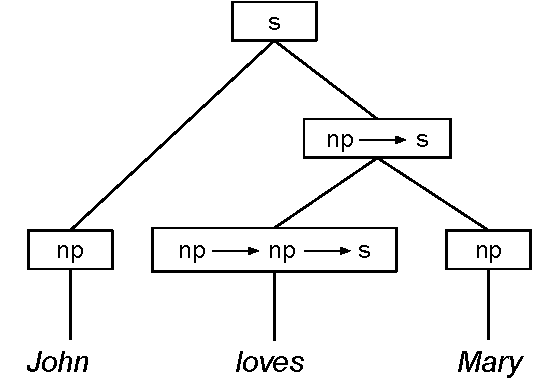
\includegraphics[width=0.4\textwidth]{images/JohnLovesMary.pdf}
\caption{Syntactic parse tree of sentence \txt{John loves Mary}.} \label{fig:JohnLovesMary-2}
\end{figure}
\begin{align}
\D = \ & \I{loves} \I{Mary} \I{John}  \notag \\
= \ & (\lambda \Y2 \X2. \X2( \lambda \x1. \Y2 (\lambda \y1. ( \lambda e' \phi. \textbf{love} \x1 \y1 \land \phi e' ))) )  \I{Mary} \I{John}  \notag \\
\bconv \ & (\lambda  \X2. \X2( \lambda \x1. \I{Mary}  (\lambda \y1. ( \lambda e' \phi. \textbf{love} \x1 \y1 \land \phi e' ))) )  \I{John}  \notag \\
\bconv \ &    \I{John}( \lambda \x1. \I{Mary}  (\lambda \y1. ( \lambda e' \phi. \textbf{love} \x1 \y1 \land \phi e' )))   \notag \\
= \ &    \I{John}( \lambda \x1. (\lambda \P2. \lambda e \phi. \P2 \textbf{m} e (\lambda e. \phi (\upii{\textbf{m}}{e'})))  (\lambda \y1. ( \lambda e' \phi. \textbf{love} \x1 \y1 \land \phi e' )))   \notag \\
\bconv \ &    \I{John}( \lambda \x1.  \lambda e \phi. (\lambda \y1. ( \lambda e' \phi. \textbf{love} \x1 \y1 \land \phi e' )) \textbf{m} e (\lambda e'. \phi (\upii{\textbf{m}}{e'})))   \notag \\
\bconv \ &    \I{John}( \lambda \x1.  \lambda e \phi. ( \lambda e' \phi. \textbf{love} \x1 \textbf{m} \land \phi e' ) e (\lambda e' . \phi (\upii{\textbf{m}}{e'})))   \notag \\
\bred \ &    \I{John}( \lambda \x1.  \lambda e \phi.  \textbf{love} \x1 \textbf{m} \land  (\lambda e' .\phi (\upii{\textbf{m}}{e'}) e))   \notag \\
\bconv \ &    \I{John}( \lambda \x1.  \lambda e \phi.  \textbf{love} \x1 \textbf{m} \land  \phi (\upii{\textbf{m}}{e} ))   \notag \\
= \ &    ( \lambda \P2. \lambda e \phi. \P2 \textbf{j} e (\lambda e' .\phi (\upii{\textbf{j}}{e'})))( \lambda \x1.  \lambda e \phi.  \textbf{love} \x1 \textbf{m} \land  \phi (\upii{\textbf{m}}{e} ))   \notag \\
\bconv \ &    \lambda e \phi. ( \lambda \x1.  \lambda e \phi.  \textbf{love} \x1 \textbf{m} \land  \phi (\upii{\textbf{m}}{e} ))   \textbf{j} e (\lambda e' . \phi (\upii{\textbf{j}}{e'})) \notag \\
\bred \ &    \lambda e \phi.  \textbf{love}  \textbf{j} \textbf{m} \land   (\lambda e' .\phi (\upii{\textbf{j}}{e'})) (\upii{\textbf{m}}{e} )  \notag \\
\bconv \ &    \lambda e \phi.  \textbf{love}  \textbf{j} \textbf{m} \land   \phi (\upii{\textbf{j}}{\upii{\textbf{m}}{e} })   \label{eq:2006:JohnLovesMary} 
\end{align}
\end{example}

To cope with anaphora, the context has to be accessed. This is accomplished by a special function $\selK$ of type $(\gamma \rightarrow \iota)$ that takes a context and returns an individual. The function $\selK$ is assumed to implement an anaphora resolution algorithm and to work as an oracle always retrieving the correct antecedent. This allows to interpret pronouns as shown, for example, for \txt{he} below:
\begin{align}
\I{he} =  \overbrace{\lambda \P2^{^\iota \rightarrow \gamma \rightarrow (\gamma \rightarrow o) \rightarrow o}. \lambda e^{\gamma} \phi^{\gamma \rightarrow o}. \overbrace{\overbrace{\overbrace{\P2 ( \overbrace{\selK_{he} e}^{\iota} )}^{\gamma \rightarrow (\gamma \rightarrow o) \rightarrow o} e}^{ (\gamma \rightarrow o) \rightarrow o} \ \phi }^{o}}^{(\iota \rightarrow \gamma \rightarrow (\gamma \rightarrow o) \rightarrow o) \rightarrow \gamma \rightarrow (\gamma \rightarrow o) \rightarrow o}  \label{eq:he:2006}
%\I{he} = \lambda \P2. \lambda e \phi. \P2 (\selK_{he}e)e\phi
\end{align}

\begin{example}[$\S$, \txt{He smiles at her}] \label{ex:2006:HeSmilesAtHer} The meaning of the sentence~\eqref{HeSmilesAtHer-2006} computed in accordance with the parse-tree shown in Figure~\ref{fig:ptS3-2006}  is as follows:
\enumsentence{\txt{He smiles at her.} \label{HeSmilesAtHer-2006}}
\begin{align}
\S = \ & \I{smiles\_at} \I{her} \I{he} \notag \\
 = \ & (\lambda \Y2 \X2. \X2( \lambda \x1. \Y2 (\lambda \y1. ( \lambda e' \phi. \textbf{smile} \x1 \y1 \land \phi e' ))) )  \I{her} \I{he} \notag \\
\bconv \ & (\lambda  \X2. \X2( \lambda \x1.  \I{her}  (\lambda \y1. ( \lambda e' \phi. \textbf{smile} \x1 \y1 \land \phi e' ))) ) \I{he} \notag \\
\bconv \ &   \I{he} ( \lambda \x1.  \I{her}  (\lambda \y1. ( \lambda e' \phi. \textbf{smile} \x1 \y1 \land \phi e' ))) \notag  \\
= \ &   \I{he} ( \lambda \x1.  (\lambda \P2. \lambda e \phi. \P2 (\selK_{her}e)e\phi)  (\lambda \y1. ( \lambda e' \phi. \textbf{smile} \x1 \y1 \land \phi e' ))) \notag \\
 \bconv \ &   \I{he} ( \lambda \x1.  (\lambda e \phi.  (\lambda \y1. ( \lambda e' \phi. \textbf{smile} \x1 \y1 \land \phi e' )) (\selK_{her}e)e\phi) ) \notag \\
  \bconv \ &   \I{he} ( \lambda \x1.  (\lambda e \phi.   ( \lambda e' \phi. \textbf{smile} \x1  (\selK_{her}e) \land \phi e' ) e\phi) ) \notag \\
 \bred \ &   \I{he} ( \lambda \x1.  (\lambda e \phi.  \textbf{smile} \x1  (\selK_{her}e) \land \phi e) ) \notag \\
  = \ &  (\lambda \P2. \lambda e \phi. \P2 (\selK_{he}e)e\phi) ( \lambda \x1.  (\lambda e \phi.  \textbf{smile} \x1  (\selK_{her}e) \land \phi e) ) \notag \\
\bconv \ & \lambda e \phi. ( \lambda \x1.  (\lambda e \phi.  \textbf{smile} \x1  (\selK_{her}e) \land \phi e) )  (\selK_{he}e)e\phi \notag \\
\bconv \ & \lambda e \phi.   (\lambda e \phi.  \textbf{smile}  (\selK_{he}e)  (\selK_{her}e) \land \phi e) e\phi \notag \\
\bred \ & \lambda e \phi.   \textbf{smile}  (\selK_{he}e)  (\selK_{her}e) \land \phi e \label{eq:2006:HeSmilesAtHer}
\end{align}
\end{example}

\begin{figure}[h]
 \centering
    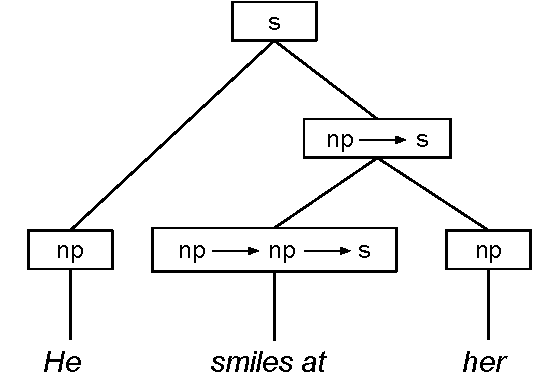
\includegraphics[width=0.4\textwidth]{images/HeSmilesatHer.pdf}
\caption{Syntactic parse tree of sentence \txt{He smiles at her}.} \label{fig:ptS3-2006}
\end{figure}

As Example~\ref{ex:2006:HeSmilesAtHer} shows, Sentence~\eqref{HeSmilesAtHer-2006} is meaningful in de~Groote's approach in the sense that it has an interpretation~\eqref{eq:2006:HeSmilesAtHer}. However, the function $\selK$ can return individuals for \txt{he} and \txt{her} only when the sentence is evaluated over some context containing the corresponding antecedents. This can be done when the sentence is uttered in a discourse and the representation of this discourse is already computed. When the meaning of the discourse is updated with the meaning of the sentence, the pronominal anaphora is resolved. 

Discourses in~\cite{deGroote:2006:Towards-a-Montagovian-Account-of-Dynamics} are, like sentences, interpreted as terms of type $(\gamma \rightarrow (\gamma \rightarrow o) \rightarrow o)$.  The update of a discourse interpreted as $\D$ with a sentence interpreted as $\S$ results in interpretation $\updt \ \D \ \S$ of a new discourse. This interpretation is defined by the following equation:
\begin{align}
\updt \ \D \ \S \defeq \overbrace{\lambda e^{\gamma} \phi^{\gamma \rightarrow o}. \overbrace{ \overbrace{\D^{\gamma \rightarrow (\gamma \rightarrow o) \rightarrow o}  e}^{(\gamma \rightarrow o) \rightarrow o} (\overbrace{\lambda e'^{\gamma}. \overbrace{\overbrace{\S^{\gamma \rightarrow (\gamma \rightarrow o) \rightarrow o}  e'}^{ (\gamma \rightarrow o) \rightarrow o} \phi}^{o}}^{\gamma \rightarrow o})}^{o}}^{\gamma \rightarrow (\gamma \rightarrow o) \rightarrow o} \label{eq:updtDS:2006}
\end{align}

\begin{example}[$\updt \ \D \ \S$]
Now interpretations~\eqref{eq:2006:JohnLovesMary} and~\eqref{eq:2006:HeSmilesAtHer} can be composed through equation~\eqref{eq:updtDS:2006}, regarding~\eqref{sent:JlovesM-2006} as the discourse updated with the sentence~\eqref{HeSmilesAtHer-2006}. This leads to the interpretation of the piece of discourse~\eqref{sen:JLMHeSH:2006}:
\enumsentence{\txt{John loves Mary. He smiles at her.} \label{sen:JLMHeSH:2006}}
\begin{align}
& \lambda e \phi. (\overbrace{\lambda e \phi.  \textbf{love}  \textbf{j} \textbf{m} \land   \phi (\upii{\textbf{j}}{\upii{\textbf{m}}{e} }) }^{\D}  ) e (\lambda e'. (\overbrace{\lambda e \phi.   \textbf{smile}  (\selK_{he}e)  (\selK_{her}e) \land \phi e}^{\S}) e' \phi ) \notag \\
\bred \ & \lambda e \phi. (\lambda e \phi.  \textbf{love}  \textbf{j} \textbf{m} \land   \phi (\upii{\textbf{j}}{\upii{\textbf{m}}{e} }) ) e (\lambda e'.  \textbf{smile}  (\selK_{he}e')  (\selK_{her}e') \land \phi e' ) \notag \\
\bred \ & \lambda e \phi.\textbf{love}  \textbf{j} \textbf{m} \land    (\lambda e'.  \textbf{smile}  (\selK_{he}e')  (\selK_{her}e') \land \phi e' )  (\upii{\textbf{j}}{\upii{\textbf{m}}{e} }) \notag \\
\bconv \ & \lambda e \phi.\textbf{love}  \textbf{j} \textbf{m} \land    \textbf{smile}  (\selK_{he}(\upii{\textbf{j}}{\upii{\textbf{m}}{e} }))  (\selK_{her}(\upii{\textbf{j}}{\upii{\textbf{m}}{e} })) \land \phi  (\upii{\textbf{j}}{\upii{\textbf{m}}{e} }) \label{int:JLMHeSH:2006}
\end{align}
\end{example}

Interpretation~\eqref{int:JLMHeSH:2006} of the discourse consisting of the utterance of~\eqref{sen:JLMHeSH:2006} is computed in a compositional manner. Note that the context of the interpretation of the first sentence is passed to $\selK$ operators of the interpretation of the second sentence. Assuming that an anaphora resolution mechanism is implemented in $\selK$, the following semantic representation of~\eqref{sen:JLMHeSH:2006} is obtained: 
\begin{align}
\lambda e \phi.\textbf{love} \  \textbf{j} \ \textbf{m} \land    \textbf{smile}  \ \textbf{j} \ \textbf{m} \land \phi  (\upii{\textbf{j}}{\upii{\textbf{m}}{e} }) \label{int:JLMHeSH:2006-2}
\end{align}
The context $(\upii{\textbf{j}}{\upii{\textbf{m}}{e} })$ in~\eqref{int:JLMHeSH:2006} (and hence in~\eqref{int:JLMHeSH:2006-2})  is accessible for future computation. This means that the individuals $\textbf{j}$ and $\textbf{m}$ can serve as ancestors for anaphoric pronouns in the following sentences. However, this is not always the case. For example, assuming accessibility constraint requirements of DRT, the individuals introduced by quantifiers in Sentence~\eqref{donkey-every-2006} should not be accessible for anaphoric triggers outside of the sentence. However, they clearly should be accessible for anaphoric pronouns within the sentence. 
\enumsentence{ \txt{Every farmer who owns a donkey beats it.} \label{donkey-every-2006}}
This accessibility constraint can also be implemented in de~Groote's approach. For example, lexical items of~\eqref{donkey-every-2006} can be assigned meanings shown in Table~\ref{tbl:donkey-lexical-2006} that lead to the desirable interpretation of the sentence, as demonstrated below. Since the lexical interpretations are dynamic, the resulting dynamic meaning of the donkey sentence does not suffer the drawbacks of the static meaning.

\begin{table}
\begin{footnotesize}
\begin{tabular}{ l l l l l }
  Lexical item & Syntactic category  & Continuation-based interpretation in {\G}\\
  \hline
  \\
  \txt{farmer} & n & $\lambda \x1 e \phi.  \cfarmer \x1 \land \phi e  $  \\
  \txt{donkey} & n & $\lambda \x1 e \phi.  \cdonkey \x1  \land \phi e  $  \\
   \txt{owns} & np $\rightarrow$ np $\rightarrow$ s & $ \lambda \Y2 \X2. \X2 ( \lambda \x1. \Y2 (\lambda \y1. ( \lambda e' \phi. \cown \x1 \y1 \land \phi e'))) $ \\
 \txt{beats} & np $\rightarrow$ np $\rightarrow$ s  & $ \lambda \Y2 \X2. \X2 ( \lambda \x1. \Y2 (\lambda \y1. ( \lambda e' \phi. \cbeat \x1 \y1 \land \phi e'))) $ \\
    \txt{a} &  n $\rightarrow$ np & $ \lambda \P2 \Q2. \lambda e \phi. \exists (\lambda \x1. \P2  \x1 e ( \lambda e'. \Q2 \x1  (\upii{\x1}{e'}) \phi ) ) $ \\
    \txt{every} & n $\rightarrow$ np & $ \lambda \P2 \Q2. \lambda e \phi. (\forall \x1. \neg (\P2 \x1 e (\lambda e'. \neg (\Q2 \x1 (\upii{\x1}{e'})  (\lambda e'''. \top)  ))))  \land \phi e$ \\
   \txt{who} & (np~$\rightarrow$~s)~$\rightarrow$~n~$\rightarrow$~n & $\lambda \R2 \Q2 \x1. \lambda e \phi. \Q2 \x1 e (\lambda e'. \R2 (\lambda \P2. \P2 \x1) e' \phi)$ \\
   \txt{it} & np & $ \lambda \P2. \lambda e \phi. \P2 ( \selK_{it} e) e \phi  $  
   \end{tabular}
\caption{Continuation-based interpretations of lexical items of the sentence \txt{Every farmer who owns a donkey beats it} in framework {\G}.} \label{tbl:donkey-lexical-2006}
\end{footnotesize}
\end{table}


\begin{example}[\txt{Every farmer who owns a donkey beats it}]
The meaning of the noun phrase \txt{a donkey} is computed by reducing the term $\trr{\I{a}} \trr{\I{donkey}} $:
\begin{align}
 \trr{\I{a}} \trr{\I{donkey}} 
 = \  & ( \lambda \P2 \Q2. \lambda e \phi. \exists (\lambda \y1. \P2  \y1 e ( \lambda e'. \Q2 \y1  (\upii{\y1}{e'}) \phi ) ) ) \trr{\I{donkey}} \notag \\ 
\bconv \ &  \lambda  \Q2. \lambda e \phi. \exists (\lambda \y1. \trr{\I{donkey}}  \y1 e ( \lambda e'. \Q2 \y1  (\upii{\y1}{e'}) \phi ) )  \notag \\ 
= \ &   \lambda  \Q2. \lambda e \phi. \exists (\lambda \y1. (\lambda \x1 e \phi.  \cdonkey \x1  \land \phi e )  \y1 e ( \lambda e'. \Q2 \y1  (\upii{\y1}{e'}) \phi ) )  \notag \\ 
\bconv \ & \lambda  \Q2. \lambda e \phi. \exists (\lambda \y1. (\lambda  e \phi.  \cdonkey \y1  \land \phi e )   e ( \lambda e'. \Q2 \y1  (\upii{\y1}{e'}) \phi ) )  \notag \\ 
\bred \  & \lambda  \Q2. \lambda e \phi. \exists (\lambda \y1.  \cdonkey \y1  \land  ( \lambda e'. \Q2 \y1  (\upii{\y1}{e'}) \phi ) e )  \notag \\ 
\bconv \  &  \lambda  \Q2. \lambda e \phi. \exists (\lambda \y1.  \cdonkey \y1  \land  \Q2 \y1  (\upii{\y1}{e}) \phi )  \label{eq:adonkey-nf-computed-2006}
\end{align}
Note that in Equation~\eqref{eq:adonkey-nf-computed-2006} the environment passed as an argument to $\Q2$ contains the variable $\y1$ introduced by the existential quantifier. This means that this variable is available to the formula $\Q2$. 
Note also that the continuation $\phi$ of the term~\eqref{eq:adonkey-nf-computed-2006}  is within the scope of the existential quantifier. 

The meaning of the verb phrase \txt{owns a donkey} is computed by $\beta$-reducing the term $  \trr{\I{owns}}  (\trr{\I{a}} \trr{\I{donkey}} )  $:
\begin{align*}
& \trr{\I{owns}}  (\trr{\I{a}} \trr{\I{donkey}} ) \\
= \ & ( \lambda \Y2 \X2. \X2 ( \lambda \x1. \Y2 (\lambda \y1. ( \lambda e' \phi. \cown \x1 \y1 \land \phi e'))) ) (\trr{\I{a}} \trr{\I{donkey} } )  \\
\bconv \ &  \lambda  \X2. \X2 ( \lambda \x1. (\trr{\I{a}} \trr{\I{donkey} } )  (\lambda \y2. ( \lambda e' \phi. \cown \x1 \y1 \land \phi e')))  \\
= \ & \lambda  \X2. \X2 ( \lambda \x1. ( \lambda  \Q2. \lambda e \phi. \exists (\lambda \y1.  \cdonkey \y1  \land  \Q2 \y1  (\upii{\y1}{e}) \phi )  )  (\lambda \y1. ( \lambda e' \phi. \cown \x1 \y1 \land \phi e')))  \\
\bconv \ &   \lambda  \X2. \X2 ( \lambda \x1. ( \lambda e \phi. \exists (\lambda \y1.  \cdonkey \y1  \land  (\lambda \y1. ( \lambda e' \phi. \cown \x1 \y1 \land \phi e')) \y1  (\upii{\y1}{e}) \phi )  )  )  \\
\bred \ &    \lambda  \X2. \X2 ( \lambda \x1. ( \lambda e \phi. \exists (\lambda \y1.  \cdonkey \y1  \land  \cown \x1 \y1 \land \phi (\upii{\y1}{e}) )  )  )  
\end{align*}
The dynamic meaning of the relative clause \txt{who owns a donkey} is computed as follows:
\begin{align}
& \trr{\I{who}}  (\trr{\I{owns}}  (\trr{\I{a}} \trr{\I{donkey}} )) \notag \\
= \ &  (\lambda \R2 \Q2 \x1. \lambda e \phi. \Q2 \x1 e (\lambda e'. \R2 (\lambda \P2. \P2 \x1) e' \phi)) (\trr{\I{owns}}  (\trr{\I{a}}  \trr{\I{donkey}} )) \notag \\
\bconv \ &  \lambda  \Q2 \x1. \lambda e \phi. \Q2 \x1 e (\lambda e'. (\trr{\I{owns}}  (\trr{\I{a}} \ \trr{\I{donkey}} ))  (\lambda \P2. \P2 \x1) e' \phi) \notag \\
= \ &   \lambda  \Q2 \x1. \lambda e \phi. \Q2 \x1 e (\lambda e'. (   \lambda  \X2. \X2 ( \lambda \x1. ( \lambda e \phi. \exists (\lambda \y1.  \cdonkey \y1  \land  \cown \x1 \y1 \land \phi (\upii{\y1}{e}) )  )  )  )  (\lambda \P2. \P2 \x1) e' \phi) \notag \\
\bconv \ &  \lambda  \Q2 \x1. \lambda e \phi. \Q2 \x1 e (\lambda e'.  (\lambda \P2. \P2 \x1) ( \lambda \x1. ( \lambda e \phi. \exists (\lambda \y1.  \cdonkey \y1  \land  \cown \x1 \y1 \land \phi (\upii{\y1}{e}) )  )  )    e' \phi) \notag \\
\bconv \ &  \lambda  \Q2 \x1. \lambda e \phi. \Q2 \x1 e (\lambda e'.   ( \lambda \x1. ( \lambda e \phi. \exists (\lambda \y1.  \cdonkey \y1  \land  \cown \x1 \y1 \land \phi (\upii{\y1}{e}) )  )  ) \x1    e' \phi) \notag \\
\bconv \ &  \lambda  \Q2 \x1. \lambda e \phi. \Q2 \x1 e (\lambda e'.  ( \lambda e \phi. \exists (\lambda \y1.  \cdonkey \y1  \land  \cown \x1 \y1 \land \phi (\upii{\y1}{e}) )  )     e' \phi) \notag \\
\bred \ &  \lambda  \Q2 \x1. \lambda e \phi. \Q2 \x1 e (\lambda e'.  \exists (\lambda \y1.  \cdonkey \y1  \land  \cown \x1 \y1 \land \phi (\upii{\y1}{e'}) )  )    \label{eq:whoownsadonkey-nf-2006}
\end{align}
The meaning of \txt{farmer who owns a donkey} is computed by applying the $\lambda$-term~\eqref{eq:whoownsadonkey-nf-2006} to the lexical interpretation of \txt{farmer}:
\begin{align*}
& (\trr{\I{who}}  (\trr{\I{owns}}  (\trr{\I{a}}  \trr{\I{donkey}} ) ) )\trr{\I{farmer}} \\
 = \ &  (  \lambda  \Q2 \x1. \lambda e \phi. \Q2 \x1 e (\lambda e'.  \exists (\lambda \y1.  \cdonkey \y1  \land  \cown \x1 \y1 \land \phi (\upii{\y1}{e'}) )  ) ) \trr{\I{farmer}}  \\
 \bconv \ &   \lambda   \x1. \lambda e \phi.  \trr{\I{farmer}}  \x1 e (\lambda e'.  \exists (\lambda \y1.  \cdonkey \y1  \land  \cown \x1 \y1 \land \phi (\upii{\y1}{e'}) )  ) \\
 = \ &    \lambda   \x1. \lambda e \phi.  (\lambda \x1 e \phi.  \cfarmer \x1 \land \phi e) \x1 e (\lambda e'.  \exists (\lambda \y1.  \cdonkey \y1  \land  \cown \x1 \y1 \land \phi (\upii{\y1}{e'}) )  ) \\
\bconv \ & \lambda   \x1. \lambda e \phi.  (\lambda  e \phi.  \cfarmer \x1 \land \phi e)  e (\lambda e'.  \exists (\lambda \y1.  \cdonkey \y1  \land  \cown \x1 \y1 \land \phi (\upii{\y1}{e'}) )  ) \\
\bred \ & \lambda   \x1. \lambda e \phi. \cfarmer \x1 \land  (\lambda e'.  \exists (\lambda \y1.  \cdonkey \y1  \land  \cown \x1 \y1 \land \phi (\upii{\y1}{e'}) )  ) e   \\
\bconv \ &  \lambda   \x1. \lambda e \phi. \cfarmer \x1 \land   \exists (\lambda \y1.  \cdonkey \y1  \land  \cown \x1 \y1 \land \phi (\upii{\y1}{e}) )         
\end{align*}
The dynamic meaning of the noun phrase \txt{every farmer who owns a donkey} is computed by applying the meaning of \txt{every} to the meaning of \txt{farmer who owns a donkey}.  
%\begin{footnotesize}
\begin{align}
& \trr{\I{every}}  ((\trr{\I{who}}  (\trr{\I{owns}}  (\trr{\I{a}}  \trr{\I{donkey}} ) )) \trr{\I{farmer}}  )  \notag \\
= \ & ( \lambda \P2 \Q2. \lambda e \phi. (\forall \x1. \neg (\P2 \x1 e (\lambda e'. \neg (\Q2 \x1 (\upii{\x1}{e'})  (\lambda e'''. \top)  ))))  \land \phi e) \notag \\
&  ((\trr{\I{who}}  (\trr{\I{owns}}  (\trr{\I{a}} \ \trr{\I{donkey}} ) )) \trr{\I{farmer}}  )   \notag \\
\bconv \ &   \lambda  \Q2. \lambda e \phi. (\forall \x1. \neg ( ((\trr{\I{who}}  (\trr{\I{owns}}  (\trr{\I{a}} \ \trr{\I{donkey}} ) )) \trr{\I{farmer}}  ) \notag \\
& \phantom{\lambda  \Q2. \lambda e \phi. (\forall \x1. \neg (} \x1 e (\lambda e'. \neg (\Q2 \x1 (\upii{\x1}{e'})  (\lambda e'''. \top)  ))))  \land \phi e  \notag \\
= \ &    \lambda  \Q2. \lambda e \phi. (\forall \x1. \neg ( (  \lambda   \x1. \lambda e \phi. \cfarmer \x1 \land   \exists (\lambda \y1.  \cdonkey \y1  \land  \cown \x1 \y1 \land \phi (\upii{\y1}{e}) )  )  \notag  \\
& \phantom{\lambda  \Q2. \lambda e \phi. (\forall \x1. \neg (} \x1 e (\lambda e'. \neg (\Q2 \x1 (\upii{\x1}{e'})  (\lambda e'''. \top)  ))))  \land \phi e  \notag \\
\bconv \ &     \lambda  \Q2. \lambda e \phi. (\forall \x1. \neg ( (  \lambda e \phi. \cfarmer \x1 \land   \exists (\lambda \y1.  \cdonkey \y1  \land  \cown \x1 \y1 \land \phi (\upii{\y1}{e}) )  )  \notag \\
& \phantom{\lambda  \Q2. \lambda e \phi. (\forall \x1. \neg (} e (\lambda e'. \neg (\Q2 \x1 (\upii{\x1}{e'})  (\lambda e'''. \top)  ))))  \land \phi e  \notag \\
\bred \ &   \lambda  \Q2. \lambda e \phi. (\forall \x1. \neg ( \cfarmer \x1 \land   \exists (\lambda \y1.  \cdonkey \y1  \land  \cown \x1 \y1 \land  \notag \\
& \phantom{\lambda  \Q2. \lambda e \phi. (\forall \x1. \neg ( \cfarmer \x1 \land   \exists (\lambda \y1.  \cdonkey \y1  \land  \cown}
(\lambda e'. \neg (\Q2 \x1 (\upii{\x1}{e'})  (\lambda e'''. \top)  )) (\upii{\y1}{e}) ) ))  \land \phi e  \notag \\
\bconv \ &   \lambda  \Q2. \lambda e \phi. (\forall \x1. \neg ( \cfarmer \x1 \land   \exists (\lambda \y1.  \cdonkey \y1  \land  \cown \x1 \y1 \land  \neg (\Q2 \x1 (\upii{\x1}{\upii{\y1}{e}})  (\lambda e'''. \top)  ) ) ))  \land \phi e  \label{eq:everyfarmerwhoownsadonkey-nf-2006}
\end{align}


Note that in Equation~\eqref{eq:everyfarmerwhoownsadonkey-nf-2006} the environment containing all the individuals with their properties collected during the computation is locally passed to the formula $\Q2$. The continuation $\phi$ receives only the environment $e$ that is passed to the term as an argument; therefore, all individuals collected during the computation of the meaning of \txt{every farmer who owns a donkey} are not available outside the logical formula interpreting this phrase.

The meaning of the verb phrase \txt{beats it} is computed as follows:
\begin{align}
 \trr{\I{beats}}  \trr{\I{it}}  
 = \ &  (\lambda \Y2 \X2. \X2 ( \lambda \x1. \Y2 (\lambda \y1. ( \lambda e' \phi. \cbeat \x1 \y1 \land \phi e')))) \trr{\I{it}}   \notag \\
 \bconv \ & \lambda  \X2. \X2 ( \lambda \x1. \trr{\I{it}}  (\lambda \y1. ( \lambda e' \phi. \cbeat \x1 \y1 \land \phi e')))   \notag \\
 = \ & \lambda  \X2. \X2 ( \lambda \x1. (  \lambda \P2. \lambda e \phi. \P2 ( \selK_{it} e) e \phi )  (\lambda \y1. ( \lambda e' \phi. \cbeat \x1 \y1 \land \phi e')))   \notag \\
 \bconv \ & \lambda  \X2. \X2 ( \lambda \x1. \lambda e \phi. (\lambda \y1. ( \lambda e' \phi. \cbeat \x1 \y1 \land \phi e')) ( \selK_{it} e) e \phi )    \notag \\
 \bconv \ &  \lambda  \X2. \X2 ( \lambda \x1. \lambda e \phi.  ( \lambda e' \phi. \cbeat \x1  ( \selK_{it} e)  \land \phi e') e \phi )    \notag \\
  \bred \ &  \lambda  \X2. \X2 ( \lambda \x1. \lambda e \phi.   \cbeat \x1  ( \selK_{it} e)  \land \phi e )  \label{eq:beatsit-nf-2006}
\end{align}
Finally, the dynamic meaning of the sentence is computed by applying the \\ term~\eqref{eq:beatsit-nf-2006} to the term~\eqref{eq:everyfarmerwhoownsadonkey-nf-2006}:
\begin{align}
& \trr{\I{beats}}  \trr{\I{it}} (\trr{\I{every}}  ((\trr{\I{who}}  (\trr{\I{owns}}  (\trr{\I{a}}  \trr{\I{donkey}} ) ) ) \trr{\I{farmer}}  )) \notag \\
= \ & ( \lambda  \X2. \X2 ( \lambda \x1. \lambda e \phi.   \cbeat \x1  ( \selK_{it} e)  \land \phi e )) \notag \\
&  (\trr{\I{every}}  ((\trr{\I{who}}  (\trr{\I{owns}}  (\trr{\I{a}}  \trr{\I{donkey}} ) ) ) \trr{\I{farmer}}  )) \notag \\
\bconv \ &   (\trr{\I{every}}  ((\trr{\I{who}}  (\trr{\I{owns}}  (\trr{\I{a}}  \trr{\I{donkey}} ) ) ) \trr{\I{farmer}}  ))  ( \lambda \x1. \lambda e \phi.   \cbeat \x1  ( \selK_{it} e)  \land \phi e ) \notag \\
= \ &    ( \lambda  \Q2. \lambda e \phi. (\forall \x1. \neg ( \cfarmer \x1 \land   \exists (\lambda \y1.  \cdonkey \y1  \land  \cown \x1 \y1 \land  \neg (\Q2 \x1 (\upii{\x1}{\upii{\y1}{e}})  (\lambda e'''. \top)  ) ) ))  \land \phi e ) \notag \\
&  ( \lambda \x1. \lambda e \phi.   \cbeat \x1  ( \selK_{it} e)  \land \phi e ) \notag \\
\bconv \ &    \lambda e \phi. (\forall \x1. \neg ( \cfarmer \x1 \land   \exists (\lambda \y1.  \cdonkey \y1  \land  \cown \x1 \y1 \land \notag \\
& \phantom{aaaaaaaaaa}  \neg (( \lambda \x1. \lambda e \phi.   \cbeat \x1  ( \selK_{it} e)  \land \phi e ) \x1 (\upii{\x1}{\upii{\y1}{e}})  (\lambda e'''. \top)  ) ) ))  \land \phi e    \notag \\
\bconv \ &  \lambda e \phi. (\forall \x1. \neg ( \cfarmer \x1 \land   \exists (\lambda \y1.  \cdonkey \y1  \land  \cown \x1 \y1 \land \notag \\
& \phantom{aaaaaaa} \neg (( \lambda e \phi.   \cbeat \x1  ( \selK_{it} e)  \land \phi e ) (\upii{\x1}{\upii{\y1}{e}})  (\lambda e'''. \top)  ) ) ))  \land \phi e    \notag \\
\bred \ &  \lambda e \phi. (\forall \x1. \neg ( \cfarmer \x1 \land   \exists (\lambda \y1.  \cdonkey \y1  \land  \cown \x1 \y1 \land \notag \\
& \phantom{aaaaaaa} \neg (  \cbeat \x1  ( \selK_{it}  (\upii{\x1}{\upii{\y1}{e}}))  \land (\lambda e'''. \top)  (\upii{\x1}{\upii{\y1}{e}})   ) ) ))  \land \phi e    \notag \\
\bconv \ &\lambda e \phi. (\forall \x1. \neg ( \cfarmer \x1 \land   \exists (\lambda \y1.  \cdonkey \y1  \land  \cown \x1 \y1 \land  \neg (  \cbeat \x1  ( \selK_{it}  (\upii{\x1}{\upii{\y1}{e}}))  \land  \top  ) ) ))  \land \phi e     \label{eq:donkey-nf-meaning-2006}
\end{align}

The resulting dynamic interpretation~\eqref{eq:donkey-nf-meaning-2006} of the donkey sentence is logically equivalent to~\eqref{eq:donkey-nf-meaning-2-2006}:
\begin{align}
 \lambda e \phi. \forall ( \lambda \x1.  \cfarmer \x1  \rightarrow    \forall ( \lambda \y1.  ( \cdonkey \y1 \land  \cown \x1 \y1 ) \rightarrow   \cbeat \x1  ( \selK_{it} (\y1 :: \x1 :: e))  )  ) )  \land \phi e  \label{eq:donkey-nf-meaning-2-2006}
\end{align}
Note that, in accordance with DRT's accessibility constraint, the individuals bound by quantifiers are not accessible outside the sentence. 
\end{example}

%The dynamic formula~\eqref{eq:donkey-nf-meaning-2-2006}, computed using the dynamic lexical interpretations, does not have the drawbacks of the static formula~\eqref{eq:donkey-st-meaning}, computed using the static lexical interpretations. 

First of all, the second argument of $\cbeat$, standing for the anaphoric pronoun, is not a free dummy variable, but a term $( \selK_{it} (\y1 :: \x1 :: e))$. This term consists of the selection function $\selK$ that takes as argument a context containing the available individuals ``collected'' during the computation. Thus, in contrast to the static case, the second argument of $\cbeat$ is self-sufficient: the function $\selK$, which implements an anaphora resolution algorithm, selects a required individual from the context. In the current case, the selection function returns the individual $\y1$, leading to the final dynamic meaning~\eqref{eq:donkey-nf-meaning-3-2006} of Sentence~\eqref{donkey-every-2006}:
\begin{align}
\lambda e \phi. \forall ( \lambda \x1.  \cfarmer \x1  \rightarrow    \forall ( \lambda \y1.  ( \cdonkey \y1 \land  \cown \x1 \y1 ) \rightarrow   \cbeat \x1 \y1  ) )  \land \phi e  \label{eq:donkey-nf-meaning-3-2006}
\end{align}

Moreover, in the dynamic interpretation, unlike in the static one, the formula $\cbeat \x1 \y1 $ is within the scope of the quantifier binding the variable $y$, exactly as desired.  Furthermore, the quantifier binding $y$ has been changed during the computation from existential to universal, which is also impossible in the static approach. These improvements are the consequences of employing a continuation-passing technique. 

The list below summarizes the advantages that de~Groote's approach brought to compositional semantics:

\begin{itemize}

\item The approach is independent of the intermediate language used to express meanings of the expressions. This allows to use mathematical and logical theories developed outside computational linguistics.\footnote{An extension of first logic language with $\lambda$ is used here because it is convenient and intuitive.} Therefore, natural language phenomena can be explained in terms of well-established and well-understood theories.

\item Variables do not have any special status and are variables in the usual mathematical sense. Therefore, the notions of free and bound variables are standard.  

\item There is no imperative dynamic notions as assignment functions, therefore destructive assignment problem does not hold. Meanings assigned to expressions are closed $\lambda$-terms. 

\item There is no need for rules that artificially extend the scope of quantifiers.

\item Context and content are regarded separately, but they do interact during the computation of the meaning of discourse.  

\item The approach does not depend on any specific structure given to the context. In contrast, context is defined as a term of type parameter $\gamma$ and, therefore, its structure can be altered when necessary.

\item The approach is truly compositional: the meaning of a complex expression is computed by $\beta$-reducing the composition of the meanings of its lexical items.

\end{itemize}

\section{The underlying dynamic logic} \label{sec:dyn_log}

It is possible to define semantics discussed in Section~\ref{sec:cont_based_dyn} in a more concise and systematic way. This is achieved by defining a continuation-based dynamic logic and this section presents this logic.

\subsection{Formal Details}

Terms and types are given by Definitions~\ref{def:terms-FO} and~\ref{def:types-FO}:
\begin{definition}[$\lambda$-terms]\label{def:FO-lambda-terms}
 The set of \textbf{$\lambda$-terms} $\Lambda$ is constructed from an enumerable set of variables $V = \{ v, v_1, v_2, \dots \}$, logical constants $\land, \exists, \neg$, two special constants $::$ and $\selK$, an enumerable set of predicate symbols $R = \{ R_1, R_2, \dots  \}$ and an enumerable set of constants $K = \{ c, c_1, c_2, \dots \}$  using application and (function) abstraction:
\begin{center}
$
\begin{array}{rcl}
x \in V & \Longrightarrow & x \in \Lambda\\
c \in K & \Longrightarrow & c \in \Lambda\\
M,N \in \Lambda &  \Longrightarrow & (MN) \in \Lambda\\ 
 x \in V, M \in \Lambda&  \Longrightarrow  & (\lambda x.M) \in \Lambda \\
  M \in \Lambda&  \Longrightarrow  & (\exists M) \in \Lambda\\ 
M,N \in \Lambda &  \Longrightarrow  & (M \land N) \in \Lambda \\
M \in \Lambda &  \Longrightarrow  & (\neg M)  \in \Lambda \\
M,x \in \Lambda &  \Longrightarrow  & (M::x) \in \Lambda\\
M \in \Lambda &  \Longrightarrow  & (\selK(M))  \in \Lambda
\end{array} 
$
\end{center}
\label{def:terms-FO}
\end{definition}

%M,x \in \Lambda &  \Longrightarrow  & (\updtfo(M,x))  \in \Lambda\\
%M \in \Lambda &  \Longrightarrow  & (\selK(M))  \in \Lambda\\


\begin{definition}[Free variables] The set of \textbf{free variables} of $t$, $FV(t)$, is defined inductively as follows:
\begin{align*}
FV(x) = \ &  \{ x \} \\
FV(c) = \ & \{ \} \\
%FV(\exists M) =  \ & FV(M) \\
%FV(M \land N) = \ & FV(M) \cup FV(N)  \\
%FV(\neg M) =  \ & FV(M) \\
%FV( \updtfo (M,x)) = \ &  FV(M) \cup FV(x)  \\
%FV(\selK(M)) = \ & FV(M) \\
FV(M N) = \ & FV(M) \cup FV(N)  \\
FV( \lambda x. M) = \ & FV(M) - \{ x \}
\end{align*}
\end{definition}

\begin{definition}[Types]
The set $\Types$ of types is defined inductively as follows:
\begin{center} $
\begin{array}{rll}
\text{Atomic types:} & \iota \in \Types & \text{(static individuals)} \\
 & o \in \Types &  \text{(static propositions)} \\
&  \gamma \in \Types &  \text{(context)} \\\\
 \text{Complex types:} & \alpha, \beta \in \Types \Longrightarrow & (\alpha \rightarrow \beta) \in \Types \\
\end{array} 
$ \end{center}
\label{def:types-FO}
\end{definition}

Typing rules define typing relations between terms and types:
\begin{definition}[Typing rules] A statement $t:\delta$, meaning $t$ has type $\delta$, is \textbf{derivable} from the basis $\Delta$, i.e. $\Delta \vdash t: \delta$, if $\Delta \vdash t: \delta$ can be produced using the following rules:

\begin{prooftree}
\AXC{} \RightLabel{axiom}
\UIC{$\Gamma, x: \alpha \vdash x: \alpha $}
\end{prooftree}

\begin{prooftree}
\AXC{} \RightLabel{axiom}
\UIC{$\Gamma \vdash \top: o $}
\end{prooftree}

\begin{prooftree}
\AXC{} %\RightLabel{axiom}
\UIC{$\Gamma, M: o, N:o \vdash M \land N: o $}
\end{prooftree}

\begin{prooftree}
\AXC{} %\RightLabel{axiom}
\UIC{$\Gamma, M: \iota \rightarrow o \vdash \exists M: o $}
\end{prooftree}

\begin{prooftree}
\AXC{} %\RightLabel{axiom}
\UIC{$\Gamma, M: o \vdash \neg M: o $}
\end{prooftree}

\begin{prooftree}
\AXC{} %\RightLabel{axiom}
\UIC{$\Gamma, c: \gamma \vdash \selK \ c:  \iota $}
\end{prooftree}

\begin{prooftree}
\AXC{} %\RightLabel{axiom}
\UIC{$\Gamma, i: \iota, c: \gamma \vdash (i::c) :  \gamma$}
\end{prooftree}


\begin{prooftree}
\AXC{} \RightLabel{axiom}
\UIC{$\Gamma \vdash c_{iv}:   \iota \rightarrow o $}
\end{prooftree}


\begin{prooftree}
\AXC{} \RightLabel{axiom}
\UIC{$\Gamma \vdash c_{tv}:   \iota \rightarrow \iota \rightarrow o $}
\end{prooftree}

\begin{prooftree}
\AXC{} \RightLabel{axiom}
\UIC{$\Gamma \vdash c_{n}:   \iota \rightarrow o $}
\end{prooftree}

\begin{prooftree}
\AXC{} \RightLabel{axiom}
\UIC{$\Gamma \vdash c_{np}:   (\iota \rightarrow o) \rightarrow o $}
\end{prooftree}

%\begin{prooftree}
%\AXC{} \RightLabel{axiom}
%\UIC{$\Gamma \vdash c_{det}:   (\iota \rightarrow o) \rightarrow ( ( \iota \rightarrow o ) \rightarrow o  )$}
%\end{prooftree}

\begin{prooftree}
\AXC{} \RightLabel{axiom}
\UIC{$\Gamma \vdash c_{rp}:  (  ((\iota \rightarrow o) \rightarrow o)  \rightarrow o)  \rightarrow   ( \iota \rightarrow o ) \rightarrow ( \iota \rightarrow o )$}
\end{prooftree}


\begin{prooftree}
\AXC{$\Gamma \vdash v: \alpha \rightarrow \beta$}
\AXC{$\Gamma \vdash u: \alpha$} \RightLabel{app}
\BIC{$\Gamma \vdash vu: \beta$}
\end{prooftree}

\begin{prooftree}
\AXC{$\Gamma, x: \alpha \vdash v:\beta$} \RightLabel{abs}
\UIC{$\Gamma \vdash \lambda x.v: \alpha \rightarrow \beta$}
\end{prooftree}
where $c_{tv}$,  $c_{iv}$, $c_{n}$, $c_{np}$ and $c_{rp}$ are constants standing for transitive and intransitive  verbs, nouns, noun phrases and relative pronouns respectively. Typing rules for other syntactic categories can be added analogously.

\end{definition}

The first axiom and the two rules (application and abstraction) are standard typing relations in simply-typed lambda calculus. The second axiom determines the type of the logical $\top$ symbol. The constant $\selK$ has type $(\gamma \rightarrow \iota)$ and the constant $::$ has type $(\iota \rightarrow \gamma \rightarrow \gamma)$. 

Each static type can be dynamized in the following way:
\begin{definition}[Dynamization of types]\label{def:DTypes-FO} Let $\iota$ and $o$ be atomic types, $\gamma$ be a type parameter, $\alpha$ and $\beta$ be arbitrary types. Then the types are \textbf{dynamized} in the following way:
\begin{subequations}
\begin{align}
\tr{\iota} \defeq \ &  \iota  \label{def:DTypes-FO:iota}\\
 \tr{o} \defeq \ & \gamma \rightarrow (\gamma \rightarrow o) \rightarrow o \label{def:DTypes-FO:o}\\
  \tr{\alpha \rightarrow \beta} \defeq \ & \tr{\alpha}  \rightarrow \tr{\beta} \label{def:DTypes-FO:atob}
\end{align}
\end{subequations}
\end{definition}
Note that the type $o$ of a static proposition is transformed to type $(\gamma \rightarrow (\gamma \rightarrow o) \rightarrow o)$. Type $(\gamma \rightarrow (\gamma \rightarrow o) \rightarrow o)$ is thus the type of a dynamic proposition. Therefore, dynamic propositions are functions from $\gamma$ (type of context) and $(\gamma \rightarrow o)$ (type of continuation) to $o$ (type of static proposition).
Static and dynamic individuals are defined to have the same type.

For each logical constant ($\neg$, $\land$ and $\exists$), its dynamic counterpart is specified by the following definition: 
\begin{definition}[Dynamic logical constants] \label{def:DLCnst-FO} Let $\A2$ and $\B2$ be terms of type $(\gamma \rightarrow (\gamma \rightarrow o) \rightarrow o)$, $\P2$ be the term of type $(\iota \rightarrow \gamma \rightarrow (\gamma \rightarrow o) \rightarrow o)$, $e$ and  $e'$ be terms of type $\gamma$, $\phi$ be a term of type $(\gamma \rightarrow o)$, $\x1$ be the term of type $\iota$. \textbf{Dynamic negation, conjunction and existential quantification} are defined respectively as follows:
\begin{subequations}
\begin{align}
\n2 \A2 \defeq \ & \lambda e \phi. \neg (\A2 e (\lambda e'. \top) ) \land \phi e  \label{def:DLCnst-FO-neg} \\
\A2 \cnj2 \B2 \defeq \ & \lambda e\phi. \A2 e (\lambda e'. \B2 e' \phi) \label{def:DLCnst-FO-cnj} \\
\ex2 ( \lambda \x1. \P2[\x1]) \defeq \ & \lambda e \phi. \exists ( \lambda \x1. \P2 [\x1] \ (x::e) \ \phi )\label{def:DLCnst-FO-ex} 
\end{align}
\end{subequations}
\end{definition}
Dynamic negation of a dynamic proposition $\A2$, $\n2 \A2$, is an abbreviation used for the term shown in~\eqref{def:DLCnst-FO-neg}. Within the body of this term, the continuation and context of $\A2$ are ``erased'' (by giving the term $(\lambda e'. \top)$ as the second argument of $\A2$)\footnote{This can be more clearly seen from Corollary~\ref{cor:DL-FO-handtop}.}, the resulting static proposition is negated, and the conjunct $\phi e$ is added. Note that both $\phi$ and $e$ are variables bound by $\lambda$. Therefore, the context of $\A2$ is not available to the continuation of the resulting term $\n2 \A2$. % and thus sentences as~\eqref{sen:itisred} are considered infelicitous:\footnote{It is a common practice to ``reject'' sentences as~\eqref{sen:itisred} by simply not providing interpretations for them. For example, according to DRT, there is no suitable marker available as an antecedent for \txt{it} in the context (remember that the content and context are represented by the same structure) and DRT does not explain how to proceed in this case. DPL and DMG require prior indexing and it is not clear which index should be assigned to \txt{it}. However, when a human being tries to comprehend sentences like~\eqref{sen:itisred}, it is resonable to assume that he/she must first interpret them (into some internal mental representation) before realizing that there is something wrong (i.e. that he/she cannot resolve the anaphora for \txt{it}). Therefore, under this assumption, frameworks that fail to provide interpretations for sentences like~\eqref{sen:itisred} can be considered flawed.}
%\enumsentence{?\txt{John does not have a car and it is red.} \label{sen:itisred}}
Dynamic existentially quantified term $\ex2 ( \lambda \x1. \P2[\x1]) $ is an abbreviation for the term shown in~\eqref{def:DLCnst-FO-ex}. It has a $\lambda$-abstraction over variables $e$ and $\phi$ and an existentially quantified variable $\x1$. Its body contains $\P2[\x1]$, which is given $e$ updated with $\x1$, $(x::e)$, and $\phi$ as arguments.  Note that $\n2$ and $\ex2$ are defined respectively via $\neg$ and $\exists$.
Dynamic conjunction is defined as a composition of two dynamic terms. The logical conjunction of static propositions is provided by the fact that each dynamic proposition has a conjunct $\phi e $ in its body, as defined in~\eqref{def:DTerms-FO-P} of the next definition.

 Given dynamic logical connectives, all static terms can be dynamized:
\begin{definition}[Dynamization of terms]\label{def:DTerms-FO} Let $\P1$ be a term of type $(\iota_1 \rightarrow \dots \rightarrow \iota_n \rightarrow o)$, $\A1$ and $\B1$ be terms of type $o$, $\t1_1, \dots, \t1_n$ and $\x1$ be terms of type $\iota$. Then propositions, negated propositions, conjunctions of two propositions and existentially quantified propositions are dynamized in the following way:
\begin{subequations}
\begin{align}
\tr{ \P1 \t1_1 \dots \t1_n } \defeq \ & \lambda e \phi . \P1 \t1_1 \dots \t1_n \land \phi e  \label{def:DTerms-FO-P}\\
\tr{ \neg \A1  } \defeq \ & \n2 \tr{\A1}  \label{def:DTerms-FO-neg}\\
\tr{ \A1 \land \B1} \defeq \ & \tr{\A1} \cnj2 \tr{\B1}  \label{def:DTerms-FO-cnj}\\
\tr{\exists( \lambda \x1. \P1 [\x1])} \defeq \ & \ex2( \lambda  \x1. \tr{\P1 [\x1]})  \label{def:DTerms-FO-ex}
\end{align}
\end{subequations}
\end{definition}
Equation~\eqref{def:DTerms-FO-P} defines the dynamization of a proposition $\P1 \t1_1 \dots \t1_n $ of type $o$ by adding a $\lambda$-abstraction with two arguments  $e$ and $\phi$  (of types $\gamma$ and $(\gamma \rightarrow o)$ respectively) and a conjunct $\phi e$. Therefore, the resulting dynamic term is of type $(\gamma \rightarrow (\gamma \rightarrow o) \rightarrow o )$, the type of a dynamic proposition. Equations~\ref{def:DTerms-FO-neg},~\ref{def:DTerms-FO-cnj} and~\ref{def:DTerms-FO-ex} extend dynamization to non-atomic formulas.

Note that Definitions~\ref{def:DLCnst-FO} and~\ref{def:DTerms-FO} allow representing de~Groote's~\cite{deGroote:2006:Towards-a-Montagovian-Account-of-Dynamics} (Section~\ref{sec:cont_based_dyn}) dynamic terms in a compact way.  While interpretations in~\cite{deGroote:2006:Towards-a-Montagovian-Account-of-Dynamics} explicitly show extra parameters, i.e. contexts and continuations, these new definitions make it possible to hide these parameters. Moreover, the resulting compact dynamic terms are structurally analogous to their original static counterparts and, hence, are more intuitive.

\begin{remark} In equations below, terms on the left side of $\defeq$ abbreviate respective terms on the right side:
\begin{align} 
\A2 \impK2 \B2 \defeq \ & \n2 (\A2 \cnj2 \n2 \B2) \\
\all2( \lambda \x1. \P2[\x1]) \defeq \ & \n2 \ex2 ( \lambda \x1. \n2 \P2 [\x1] )
\end{align}
\end{remark}


Proposition~\ref{thrm:scopeextension-G}  proves an important $\beta$-equivalence that can be useful when computing interpretations of certain phrases containing an existentially quantified variable.
%%%%%%%%%%%%%%%%%%%%%%%%%%%%%%%%%%%%%%%%%%%%%%%%%%%%%%%%%%%%%%%%%%%%%%%%%%%%%%%%%%%%%
%%%%%%%%%%%%%%%%%%%%%%%%%%%%%%%%%%%%%%%%%%%%%%%%%%%%%%%%%%%%%%%%%%%%%%%%%%%%%%%%%%%%%
\begin{proposition} For all terms $\A1$ and $\B1$ of type $o$ such that  $\x1 \in FV(\A1)$ and $\x1 \notin FV(\B1)$ for an $\x1$ of type~$\iota$, the following equivalence holds: \label{thrm:scopeextension-G}
\begin{align*}
  {\ex2} (\lambda \x1.  \tr{\A1[\x1]}) \cnj2 \tr{\B1}  =_{\beta}  \ex2 (\lambda \x1.  \tr{\A1[\x1]}  \cnj2  \tr{\B1} ) 
\end{align*} 
\end{proposition}
%%%%%%%%%%%%%%%%%%%%%%%%%%%%%%%%%%%%%%%%%%%%%%%%%%%%%%%%%%%%%%%%%%%%%%%%%%%%%%%%%%%%%
%
\begin{proof}
%
\begin{align}
 &  {\ex2} (\lambda \x1.  \tr{\A1[\x1]}) \cnj2 \tr{\B1}  \notag \\ 
 \bred \  &  ( \lambda e \phi.  \exists ( \lambda \x1. \A1[\x1] \land \phi (x::e) ) )  \cnj2  \tr{\B1}  \tag{by~\eqref{def:DLCnst-FO-ex}}\\
= \ &  \lambda e \phi. ( \lambda e \phi.  \exists ( \lambda \x1. \A1[\x1] \land \phi (x::e) ) ) e ( \lambda e. \tr{\B1} e \phi  ) \tag{by~\eqref{def:DLCnst-FO-cnj}} \\
\bred \ &   \lambda e \phi. ( \lambda e \phi.  \exists ( \lambda \x1. \A1[\x1] \land \phi (x::e) ) ) e ( \lambda e. \B1 \land  \phi e  )  \tag{by~\eqref{def:DTerms-FO-P}}\\
\bred \ &   \lambda e \phi.  \exists ( \lambda \x1. \A1[\x1] \land  (  \B1 \land  \phi  (x::e)  ) ) \label{eq:DLGexscope1}
\end{align}
%
\begin{align}
 &  \ex2 (\lambda \x1.  \tr{\A1[\x1]}  \cnj2  \tr{\B1} ) \notag \\
  = \ &    \ex2 (\lambda \x1.  \lambda e \phi. \tr{\A1[\x1]}  e (\lambda e. \tr{\B1}  e \phi)  ) \tag{by~\eqref{def:DLCnst-FO-cnj}} \\
  \bred \ &  \ex2 (\lambda \x1.  \lambda e \phi. (\lambda e \phi. \A1[\x1] \land \phi e ) e (\lambda e. \B1 \land  \phi e)  ) \tag{by~\eqref{def:DTerms-FO-P}}\\
    \bred \ &   \ex2 (\lambda \x1.  \lambda e \phi. \A1[\x1] \land  (\B1 \land  \phi e )   ) \\
\bred \ &   \lambda e \phi.  \exists ( \lambda \x1.   \A1[\x1] \land  (  \B1 \land  \phi ( \x1:: e ) ) ) \tag{by~\eqref{def:DLCnst-FO-ex}}
\end{align}
%
\end{proof}

\begin{proposition} For all $\h1$ and $\v1$ of type $o$, and for all $\u1$ of type $\gamma$, the following holds: $$\tr{\h1} \u1 (\lambda e.\v1) =  \h1 \land \v1$$ where $e$ is a variable of type $\gamma$. \label{DL-FO-handv}
\end{proposition}
\begin{proof}
The proof is by induction on the structure of the term $\h1$.
\begin{itemize}
\item $\h1$ is a proposition of the form $\P1 t_1 \dots t_n$.
\begin{align}
\tr{\P1 \t1_1 \dots \t1_n} \u1  (\lambda e.\v1)  = \ & (\lambda e \phi. \P1 \t1_1 \dots \t1_n \land \phi e) \u1  (\lambda e.\v1) \tag{by~\eqref{def:DTerms-FO-P}} \\
\bconv \ & (\lambda  \phi. \P1 \t1_1 \dots \t1_n \land \phi \u1)   (\lambda e.\v1) \notag \\
\bconv \ & \lambda  \phi. \P1 \t1_1 \dots \t1_n \land (\lambda e.\v1) \u1    \notag \\
\bconv \ & \lambda  \phi. \P1 \t1_1 \dots \t1_n \land \v1    \notag 
\end{align}

\item  $\h1$ is a negated proposition $ \neg \w1$. 
\begin{align}
\tr{\neg \w1} \u1 (\lambda e. \v1) = \ &  \n2 \tr{\w1}  \u1 (\lambda e. \v1)  \tag{by~\eqref{def:DTerms-FO-neg}} \\
= \ & ( \lambda e \phi. \neg (\tr{\w1} e (\lambda e'. \top) ) \land \phi e)  \u1 (\lambda e. \v1)  \tag{by~\eqref{def:DLCnst-FO-neg}} \\
\bconv \ & ( \lambda \phi.\neg (\tr{\w1} \u1 (\lambda e'. \top) ) \land \phi \u1 ) (\lambda e. \v1)  \notag \\
\bconv \ & \neg (\tr{\w1} \u1 (\lambda e'. \top) ) \land  (\lambda e. \v1) \u1   \notag \\
\bconv \ & \neg (\tr{\w1} \u1 (\lambda e'. \top) ) \land   \v1   \notag \\
= \ & \neg(\w1 \land \top) \land \v1 \tag{by I.H.} \\
= \ & \neg \w1 \land \v1
\end{align}

\item $\h1$ is a conjunction of two propositions $\w1 \land \z1$.
\begin{align}
(\tr{\w1 \land \z1}) \u1 (\lambda e. \v1)  = \ & (\tr{\w1} \cnj2 \tr{\z1}) \u1 (\lambda e. \v1)   \tag{by~\eqref{def:DTerms-FO-cnj}} \\
 = \ & (\lambda e\phi. \tr{\w1} e (\lambda e'. \tr{\z1} e' \phi) ) \u1 (\lambda e. \v1)   \tag{by~\eqref{def:DLCnst-FO-cnj}} \\
\bconv \ & (\lambda \phi. \tr{\w1} \u1 (\lambda e'. \tr{\z1} e' \phi) ) (\lambda e. \v1)   \notag \\
\bconv \ &  \tr{\w1} \u1 (\lambda e'. \tr{\z1} e'  (\lambda e. \v1) )  \notag \\
= \ &  \tr{\w1} \u1 (\lambda e'. \z1 \land \v1)  \tag{by I.H., $e \notin FV(\v1)$} \\
= \ &  \w1 \land (\z1 \land \v1)  \tag{by I.H., $e' \notin FV(\z1 \land \v1)$} \\
\logeq \ & (\w1 \land \z1) \land \v1 \notag
\end{align}

\item $\h1$ is an existentially quantified formula of the form $\exists( \lambda \x1. \P1 [\x1])$.
\begin{align}
\tr{\exists ( \lambda \x1. \P1 [\x1])} \u1 (\lambda e. \v1)  = \ & ( \ex2 ( \lambda \x1. \tr{\P1 [\x1]})  ) \u1 (\lambda e. \v1)   \tag{by~\eqref{def:DTerms-FO-ex}} \\
 = \ & ( \lambda e \phi. \exists ( \lambda \x1. \P2 [\x1] (x::e) \phi  )) \u1 (\lambda e. \v1)   \tag{by~\eqref{def:DLCnst-FO-ex}} \\
\bconv \ & ( \lambda  \phi. \exists ( \lambda \x1. \P2 [\x1] (x::\u1) \phi  ))  (\lambda e. \v1)  \notag \\
\bconv \ & \exists ( \lambda \x1. \P2 [\x1] (x::\u1) (\lambda e. \v1)  )  \notag \\
= \ & \exists ( \lambda \x1. \P1 [\x1] \land \v1  )  \tag{by I.H.} \\
= \ & \exists ( \lambda \x1. \P1 [\x1]) \land \v1    \tag{$\x1 \notin FV(\v1)$} 
\end{align}

\end{itemize}
\end{proof}

\begin{corollary} \label{cor:DL-FO-handtop} For all propositions $\t1$ of type $o$, and for all terms $\u1$ of type $\gamma$, the following folds: 
\begin{align}\tr{\t1} \u1 (\lambda e. \top) \logeq  \t1 \notag  %\label{eq:DL-FO-handtop}
\end{align}
where $e$ is a variable of type $\gamma$.
 \label{DL-FO-handtop}
\end{corollary}
\begin{proof} Take $\v1$ equal to $\top$ in Proposition~\ref{DL-FO-handv}. Then
$$\tr{\t1} \u1 (\lambda e. \top) = \t1 \land \top \logeq \t1$$
\end{proof}


\begin{definition} A dynamic proposition $\t2$ is true in a model $\mathcal{M}$, denoted
$\mathcal{M}~\models_{dyn}~\t2$, if and only if $\mathcal{M}$ $\models$ $\t2 u (\lambda e. \top)$ for every $u$ of type $\gamma$. \label{def:dyntrueinmodel}
\end{definition}

\begin{theorem}[Conservation] A proposition $\t1$ is true in a model $\mathcal{M}$  if and only if its dynamic variant $\tr{\t1}$ is true in the same model: 
 $$\mathcal{M} \models \t1 \ \text{iff} \ \mathcal{M} \models_{dyn} \tr{\t1}$$
 \label{th:conservation:FO}
\end{theorem}
\begin{proof}

If $\mathcal{M} \models \t1$, then, by Corollary~\ref{cor:DL-FO-handtop}, $\mathcal{M} \models \tr{\t1} \u1 (\lambda e.\top)$. Therefore, by Definition~\ref{def:dyntrueinmodel}, $\mathcal{M} \models_{dyn} \tr{\t1}$.

If $\mathcal{M} \models_{dyn} \tr{\t1}$, then, by Definition~\ref{def:dyntrueinmodel}, $\mathcal{M} \models \tr{\t1} \u1 (\lambda e.\top)$. Therefore, by Corollary~\ref{cor:DL-FO-handtop}, $\mathcal{M} \models \t1$.
\end{proof}

The conservation theorem proves that a static proposition and its dynamic version defined in this section hold in the same models.


\subsection{Donkey Sentences}

Tables~\ref{tbl:stat-FO-donkey} and~\ref{tbl:dyn-FO-donkey} show respectively static and dynamic (according to {\GN}) interpretations for the lexical items in the donkey sentence~\eqref{donkey-every-FO}:
\enumsentence{ \txt{Every farmer who owns a donkey beats it.} \label{donkey-every-FO}}
Note that the type of every dynamic term is analogous to its static type. The only difference is that each atomic type of a dynamic term is dynamized according to Definition~\ref{def:DTypes-FO}. All terms in Table~\ref{tbl:dyn-FO-donkey}, except the interpretation of the pronoun \txt{it}, are dynamized following the rules in Definition~\ref{def:DTerms-FO}. These rules allow the presentation of dynamic terms in a compact way. They ensure that dynamic terms are structurally analogous to their static counterparts and, therefore, are more intuitive. The dynamic interpretation of \txt{it} is constructed not by directly following the dynamization rules, because \txt{it} is a unconventional lexical item: there is an anaphor to be solved. Therefore, $\etr{\I{\txt{it}}}$\footnote{Here and further on, dynamic interpretations of unconventional lexical items are marked with tilde.} contains the selection function $\selK$ that takes a context (from which a referent has to be chosen) as an argument.

 Taking these dynamic interpretations to compute the meaning of Sentence~\eqref{donkey-every-FO}, term~\eqref{eq:FO-donkey-int0} $\beta$-reduces to term~\eqref{eq:FO-donkey-int1}, which normalizes to~\eqref{eq:FO-donkey-int1-equiv}:
\begin{align}
& \tr{\I{beats}}  \ \etr{\I{it}} (\tr{\I{every}}  ((\tr{\I{who}}  (\tr{\I{owns}}  (\tr{\I{a}} \ \tr{\I{donkey}} ) ) ) \tr{\I{farmer}}  ))  \label{eq:FO-donkey-int0} \\
\bred \ &  \all2 (\lambda \x1. (\tr{\textbf{f}} \x1  \cnj2     \ex2 (\lambda \z1.   \tr{\textbf{d}}   \z1  \cnj2      \tr{\textbf{o}}  \x1  \z1 ))    \impK2    (\lambda e \phi. \tr{\textbf{b}}  \x1 ( \selK_{it} e ) e \phi ) )  \label{eq:FO-donkey-int1} \\
\bred \ & \lambda e \phi. \forall (\lambda \x1. \cfarmer \x1  \rightarrow \forall  (\lambda \z1.  (\cdonkey  \z1 \land \cown  \x1 \z1 )   \rightarrow  \cbeat  \x1 ( \selK_{it}  (\upii{\x1}{\upii{\z1}{e}}) )))\land \phi e  \label{eq:FO-donkey-int1-equiv}
\end{align}


Resulting term~\eqref{eq:FO-donkey-int1-equiv} is equivalent to~\eqref{eq:donkey-nf-meaning-2-2006} obtained in framework {\G} interpretations. Indeed, framework {\GN} is equivalent to de Groote's~\cite{deGroote:2006:Towards-a-Montagovian-Account-of-Dynamics} framework {\G}. However, it is advantageous over {\G} due to the compact notations for dynamic terms. These notations significantly systematize the framework and make the interpretations more concise and intuitive. Moreover, the systematic translations of static terms into dynamic terms makes it possible to prove a conservation result~\ref{th:conservation:FO} for {\GN}, that guarantees that static and dynamic interpretations are satisfied in the same models. 




\begin{table}
\begin{tabular}{ l l l l }
  Lexical item &  Static type & Static interpretation \\
  \hline
  \\
  \txt{farmer} &  ${\iota} \rightarrow {o}$ &  $\textbf{f}$   \\
  \txt{donkey} &  ${\iota} \rightarrow {o}$ &  $\textbf{d}$   \\
  \txt{owns} & $((\iota \rightarrow o) \rightarrow o) \rightarrow ((\iota \rightarrow o) \rightarrow o) \rightarrow {o}$  & $ \lambda \Y1 \X1. \X1 ( \lambda \x1. \Y1 (\lambda \y1.  \textbf{o}  \x1 \y1 ))$ \\
    \txt{beats} & $((\iota \rightarrow o) \rightarrow o) \rightarrow ((\iota \rightarrow o) \rightarrow o) \rightarrow {o}$  & $ \lambda \Y1 \X1. \X1 ( \lambda \x1. \Y1 (\lambda \y1.  \textbf{b}  \x1 \y1 ))$ \\
   \txt{every} & $({\iota} \rightarrow {o}) \rightarrow ( ({\iota} \rightarrow {o}) \rightarrow {o}) $ & $\lambda \P1 \Q1. \forall (\lambda x. \P1 x \rightarrow \Q1 x ) $   \\
   \txt{a} & $({\iota} \rightarrow {o}) \rightarrow ( ({\iota} \rightarrow {o}) \rightarrow {o}) $ & $ \lambda \P1 \Q1. \exists (\lambda x.  \P1 x \land \Q1 x )$ \\
  \txt{who} & $( ( ({\iota} \rightarrow {o}) \rightarrow {o} ) \rightarrow o  )  \rightarrow (\iota \rightarrow o)  \rightarrow (\iota \rightarrow o) $ & $ \lambda \R1 \Q1 \x1. \Q1 \x1 \land \R1 (\lambda \P1. \P1 \x1) $  \\
   \txt{it} & $ ({\iota} \rightarrow {o}) \rightarrow {o} $  & $\lambda \P1. \P1 ?$ \\ 
 \end{tabular}
\caption{Static lexical interpretations.} \label{tbl:stat-FO-donkey}
\end{table}
\begin{table}
\begin{tabular}{ l l l l l}
  Lexical item & Dynamic type & Dynamic interpretation in {\GN} \\
  \hline
  \\
  \txt{farmer} &  $\tr{\iota} \rightarrow \tr{o}$ &  $\tr{\textbf{f}}$  \\
    \txt{donkey} &  $\tr{\iota} \rightarrow \tr{o}$ &  $\tr{\textbf{d}}$  \\
   \txt{owns} & $((\tr{\iota} \rightarrow \tr{o}) \rightarrow \tr{o}) \rightarrow ((\tr{\iota} \rightarrow \tr{o}) \rightarrow \tr{o}) \rightarrow \tr{o}$  & $ \lambda \Y2 \X2. \X2 ( \lambda \x1. \Y2 (\lambda \y1.  \tr{\textbf{o}}  \x1 \y1 ))$ \\
      \txt{beats} & $((\tr{\iota} \rightarrow \tr{o}) \rightarrow \tr{o}) \rightarrow ((\tr{\iota} \rightarrow \tr{o}) \rightarrow \tr{o}) \rightarrow \tr{o}$  & $ \lambda \Y2 \X2. \X2 ( \lambda \x1. \Y2 (\lambda \y1.  \tr{\textbf{b}}  \x1 \y1 ))$ \\
   \txt{every} & $(\tr{\iota} \rightarrow \tr{o}) \rightarrow ( (\tr{\iota} \rightarrow \tr{o}) \rightarrow \tr{o}) $ & $\lambda \P2 \Q2. \all2 (\lambda \x1.  \P2 \x1  \impK2 \Q2 \x1 ) $ \\
    \txt{a} &  $(\tr{\iota} \rightarrow \tr{o}) \rightarrow ( (\tr{\iota} \rightarrow \tr{o}) \rightarrow \tr{o}) $  & $ \lambda \P2 \Q2. \ex2 (\lambda \x1.  \P2 \x1  \cnj2   \Q2 \x1 )$ \\
   \txt{who} & $( ( (\tr{\iota} \rightarrow \tr{o}) \rightarrow \tr{o} ) \rightarrow \tr{o}  )  \rightarrow (\tr{\iota} \rightarrow \tr{o})  \rightarrow (\tr{\iota} \rightarrow \tr{o}) $ & $\lambda \R2 \Q2 \x1. \Q2 \x1  \cnj2  \R2 (\lambda \P2. \P2 \x1 ) $\\
      \txt{it} & $ \lambda \P2. \lambda e \phi. \P2 ( \selK_{it} e ) e \phi $ \\ 
   \end{tabular}
\caption{Dynamic lexical interpretations in framework {\GN}.} \label{tbl:dyn-FO-donkey}
\end{table}
\section{Comparison with related work} \label{sec:dpl}

Constants, variables, reference markers: $\mathsf{C}, \mathsf{V}, \mathsf{M}$

model: $\mathscr{M} = \langle D, \mathcal{I}\, \rangle$

left contexts : $\env = D^{\mathsf{M}}$

continuations : $\cont = 2^\env$ 

nota: a tdl term may contain ref. markers (this stands for $\sel{}$)

\begin{align*}
\dplsem{\app{\app{\app{R}{t_1}}{\ldots}}{t_n}} &= 
\{\langle g,h\rangle  :
h=g \,\wedge\, 
\langle 
\llbracket t_1 \rrbracket_{\eta,g},
\dots,
\llbracket t_n \rrbracket_{\eta,g}
\rangle \in \mathcal{I}(R)
\}
\\
\dplsem{\conj{P}{Q}} &= 
\{\langle g,h\rangle  : 
\equant{k}{
\langle g,k\rangle\in \dplsem{P}
\,\wedge\,
\langle k,h\rangle\in \dplsem{Q}
}\}
\\
\dplsem{\nega{P}} &=
\{\langle g,h\rangle  : 
h=g \,\wedge\, 
\uquant{k}{\langle g,k \rangle\not\in\dplsem{P}}
\}
\\
\dplsem{\equant{\mathbf{i}}{P}} &=
\{\langle g,h\rangle  : 
\equant{k}{
k[\mathbf{i}]g \,\wedge\,
\langle k,h \rangle \in \dplsem{P}
}\} 
\end{align*}

\begin{align*}
\synlift{c}_e &= c\\
\synlift{x}_e &= x\\
\synlift{\mathbf{i}}_e &= \app{\mathsf{sel}_i}{e}\\
\end{align*}

\begin{align*}
\synlift{\app{\app{\app{R}{t_1}}{\ldots}}{t_n}} &= 
\abs{e\phi}{\conj{
\app{\app{\app{R}{
\synlift{t_1}_e
}}{\ldots}}{
\synlift{t_n}_e}
}{\app{\phi}{e}}}
\\
\synlift{\conj{P}{Q}} &= 
\dconj{\synlift{P}}{\synlift{Q}}
\\
\synlift{\nega{P}} &= \dnega{\synlift{P}}
\\
\synlift{\equant{\mathbf{i}}{P}} &=
\dynexists_{\mathbf{i}} x.\,\synlift{P[\mathbf{i}{:=}x]}
\end{align*}

\begin{align*}
\tdlsem{\eta}{\app{\app{\app{R}{t_1}}{\ldots}}{t_n}} &= 
\{\langle g,H\rangle   :
g \in H \, \wedge \,
\langle 
\llbracket t_1 \rrbracket_{\eta,g},
\dots,
\llbracket t_n \rrbracket_{\eta,g}
\rangle \in \mathcal{I}(R)
\}
\\
\tdlsem{\eta}{\dconj{P}{Q}} &= 
\{\langle g,H\rangle  :
\langle g, 
\{h : \langle h, H\rangle \in \tdlsem{\eta}{Q}\}
\rangle\in\tdlsem{\eta}{P}
\}
\\
\tdlsem{\eta}{\dnega{P}} &=
\{\langle g,H\rangle  :
g \in H \, \wedge \,
\langle g,\env\rangle\not\in \tdlsem{\eta}{P}
\}
\\
\tdlsem{\eta}{\dynexists_{\mathbf{i}} x.\, P} &=
\{\langle g,H\rangle  :
\equant{a}{\langle g[\mathbf{i}{:=}a],H\rangle\in\tdlsem{\eta[x{:=}a]}{P}}
\} 
\end{align*}

$$
\semlift{\mathrm{R}} = \{\langle a,B\rangle : 
\equant{b}{\conj{b\in B}{\langle a,b\rangle\in R}}\}
$$



$$
\semlift{\dplsem{P}} = \tdlsem{\eta}{\synlift{P}}
$$

\begin{lemma}
Let $t$ be a term, and let $x$ be a variable that does not occur in $t$.
For all reference marker $\mathbf{i}$, all assignment $g$, and all valuation
$\eta$, the following holds:
$$
\llbracket t \rrbracket_{\eta,g} =
\llbracket t[\mathbf{i}{:=}x] \rrbracket_{\eta[x{:=}(\app{g}{\mathbf{i}})],g}
$$
\begin{proof}
If $t$ is a constant or a reference marker different from $\mathbf{i}$,
the result is immediate.
If $t$ is a variable $y$, we have that $y\not= x$. Consequently,
$\app{\eta}{y} = \app{\eta[x{:=}(\app{g}{i})]}{y}$.
Finally, if $t$ is $\mathbf{i}$, we have
$\llbracket \mathbf{i} \rrbracket_{\eta,g} =
\app{g}{\mathbf{i}} = 
\app{\eta[x{:=}(\app{g}{i})]}{x} = 
\llbracket x \rrbracket_{\eta[x{:=}(\app{g}{\mathbf{i}})],g} =
\llbracket\mathbf{i}[\mathbf{i}{:=}x] \rrbracket_{\eta[x{:=}(\app{g}{\mathbf{i}})],g}
$.
\end{proof}
\end{lemma}




----------------------------------------------

DPL, at least as it is presented in~\cite{GroenendijkStokhof:1991:Dynamic-Predicate-Logic} does not provide a translation from natural language to the language of DPL. In contrast, this dissertation is focused exactly on providing a translation from natural language to the language of continuation based-dynamic logic. This makes it impossible to make a direct comparison between DPL and {\GLex} (as well as its predecessors {\GN} and {\GL}). Nevertheless, it is still possible to compare the frameworks by defining certain translations between their different levels. Since, among {\GN}, {\GL} and {\GLex}, the closest to DPL w.r.t. expressive power is {\GN}, translations between {\GN} and DPL are defined subsequently.

Consider Figure~\ref{DPLscheme}. The missing translation $\ntodpl$ of natural language into the language of DPL is represented by the dashed arrow. The translation $\ntodl$ of natural language into the language $\langDL$ of continuation-based dynamic logic is represented by the green arrow.
 \begin{figure}[h!]
  \centering
    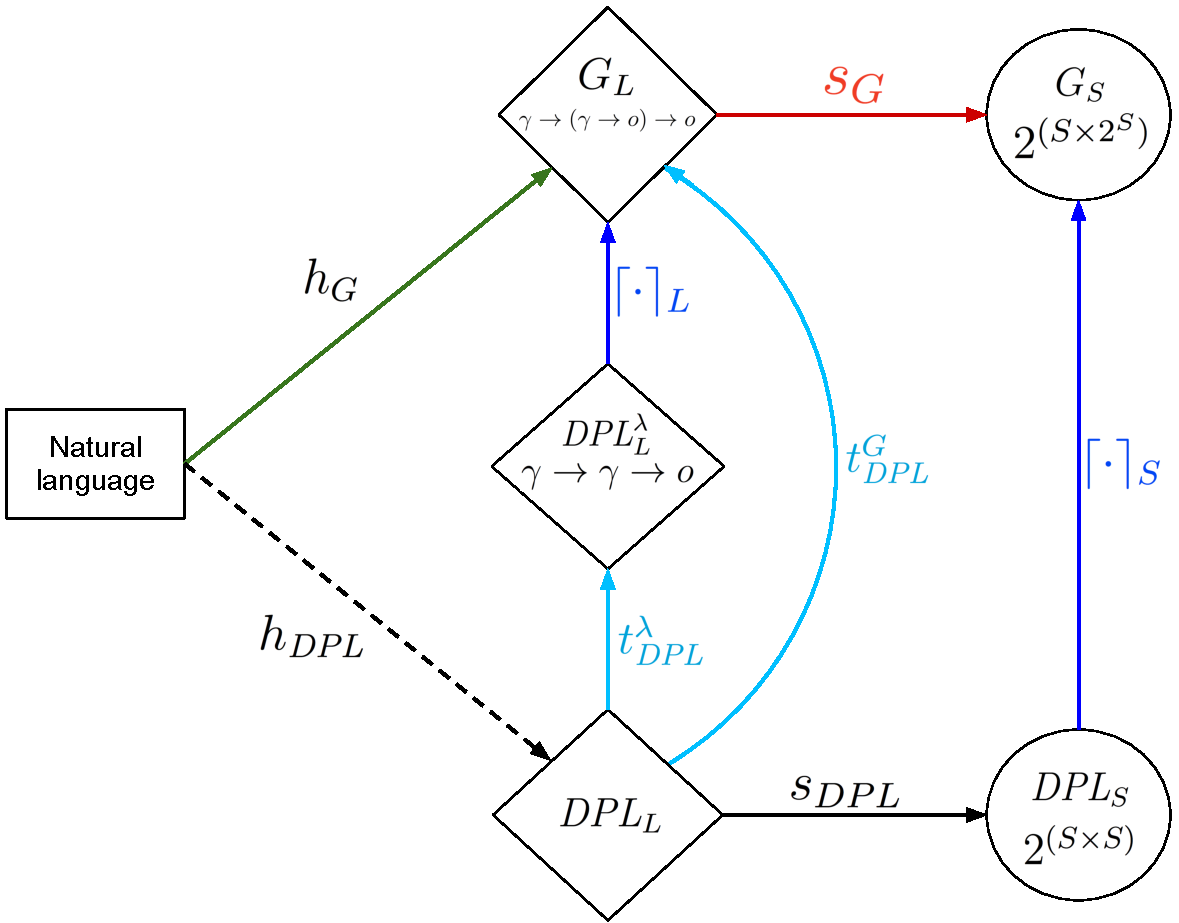
\includegraphics[width=1\textwidth]{images/DPLscheme.pdf}
      \caption{Comparison between DPL and {\GN}.} \label{DPLscheme}
\end{figure}

What Groenendijk and Stokhof~\cite{GroenendijkStokhof:1991:Dynamic-Predicate-Logic} define is a translation $\dpltos$ of the language of DPL into binary relations on states $\statesDPL$. This translation is illustrated with the black solid arrow.

There are two possible ways to compare DPL and {\GN}. One possibility is to define a translation $\dltos$ (red arrow) of the language of {\GN} into relations on states $\statesDL$ and to compare  $\statesDL$ with $\statesDPL$. Another possibility is to define a translation $\dplstodpll$ (shorter light blue arrow) of the language $\langDPL$ of DPL into a new language $\newDPL$ and to compare $\newDPL$ with the language  $\langDL$ of {\GN}. These two comparisons are presented in more details below.


\subsubsection{Comparison 1}

DPL interprets propositions as binary relations on states and its semantics is defined as the following translation from $\langDPL$ to $\statesDPL$ (solid black arrow):
\begin{definition}[Translation $\dpltos$] Let $A, B$ and $P$ be terms in $\langDPL$ of type $o$. Let $h, g$ and $k$ be assignments of values to variables (a.k.a. states). Translation $\dpltos:  \langDPL \rightarrow \statesDPL$ is defined as follows:
\begin{align*}
\mdpltos{A} = \ & \{ \langle g , h \rangle \ | \ h = g \land h  \models A \} \\
\mdpltos{\neg P} = \ & \{ \langle g , h \rangle \ | \ h = g \land \neg ( \exists k.  \ \langle h, k \rangle \in  \mdpltos{P} ) \} \\
\mdpltos{A \land B} = \ & \{ \langle g , h \rangle \ |  \ \exists k. \ \langle g, k \rangle \in  \mdpltos{A}  \land   \langle k, h \rangle \in  \mdpltos{B}  \} \\
\mdpltos{\exists i. P} = \ & \{ \langle g , h \rangle \ |  \ \exists k.  \  k [i] g \land  \langle k, h \rangle \in  \mdpltos{P} \} 
\end{align*}
\end{definition}
\noindent Thus, for every proposition $P$, $\mdpltos{P}$ is in $2^{(S \times S)}$.
%

\noindent A similar translation $\dltos$ (red arrow) of propositions in $\langDL$ into relations defined on states can be defined:
\begin{definition}[Translation $\dltos$] Let $S$, the set of states, be the semantic domain that interprets $\gamma$. The translation $\dltos: \langDL \rightarrow \statesDL$ is defined as follows:
\begin{align*}
\mdltos{A} = \ & \{ \langle g , H \rangle \ | \ g \in H \land g \models A \} \\
\mdltos{\n2 P} = \ & \{ \langle g , H \rangle \ | \ g \in H \land \langle g, S \rangle \notin \mdltos{P} \} \\
\mdltos{A \cnj2 B} = \ & \{ \langle g , H \rangle \ | \ \langle g , \{ h \ | \ \langle h, H \rangle \in \mdltos{B} \} \rangle \in \mdltos{A} \} \\
\mdltos{\ex2_i x. P} = \ & \{ \langle g , H \rangle \ | \ \exists x. \langle (x,i)::g ,  H \rangle \in \mdltos{P} \} 
\end{align*}
\end{definition}
Note that  $\dltos$ interprets propositions not just as relations between states, but as relations betweens states and sets of states: for each proposition $P$, $\mdltos{P}$ is in  $2^{(S \times 2^S)}$. Therefore, $\dltos$ is richer than $\dpltos$ and avoids existentially quantified states and equality relations on states by using set inclusion.  Moreover, there exists a canonical embedding (larger blue arrow) of $\statesDPL$ into $\statesDL$:
\begin{definition}[Embedding of $\statesDPL$ into $\statesDL$] Let $R$ be set of pair of states (in $2^{(S \times S)}$) in $\statesDPL$, the embedding $\dplstodls$ of $\statesDPL$ into $\statesDL$ is as follows: 
\begin{align}
\mdplstodls{R} \defeq \ & \{  \langle g, H \rangle \ | \ \exists h. \ h \in H \land \langle g, h \rangle \in R  \} \notag
\end{align}
$\mdplstodls{R}$  is in $2^{(S \times 2^S)}$.
\end{definition}
Note that there is a correspondence between types constructed from $\gamma$ and $o$ and sets constructed from $S$ and the cross product powerset operations:
\begin{align}
 [\gamma ] \approx \ & S \notag \\
 [\alpha_1 \rightarrow \alpha_2 \rightarrow  \dots \rightarrow \alpha_n \rightarrow o] \approx \ & 2^{[\alpha_1] \times [\alpha_2] \times \dots \times [\alpha_n]} \notag
\end{align}
Consequently, the type $(\gamma \rightarrow (\gamma \rightarrow o) \rightarrow o )$ corresponds to the set $2^{(S \times 2^S)}$.

 The following translation $\dpltodl$ (longer light blue arrow) of  $\langDPL$ to  $\langDL$ can be defined:
\begin{definition}[Translation $\dpltodl$] Let $A, B$ and $P$ be propositions. The translation $\dpltodl: \langDPL \rightarrow \langDL$ is defined as follows:
\begin{align*}
 \mdpltodl{A}  = \ & A \\
 \mdpltodl{\neg P} = \ & \n2 \mdpltodl{P} \\
 \mdpltodl{ A \land B} = \ & \mdpltodl{A} \cnj2 \mdpltodl{B} \\ 
 \mdpltodl{\exists i. P} = \ & \ex2_i x. \mdpltodl{P}
\end{align*}
\end{definition}

\begin{theorem} \label{th:dplltodll} Let $P$ be a proposition. Then the following equivalence holds:
\begin{align}
 \mdplstodls{ \mdpltos{P}} = \mdltos{\mdpltodl{P}} \notag
\end{align}
by postulating
\begin{align}
g [i] h \ \  \text{iff} \  \ \exists x. (h = (x,i)::g) \notag
\end{align}
\end{theorem}
\begin{proof} The proof is by induction on the structure of $P$.
\end{proof}

By Theorem~\ref{th:dplltodll}, transforming $\langDPL$ to $\langDL$ and interpreting the result in $\statesDL$ according to $\dltos$ is equivalent to DPL's original semantics. 

\subsubsection{Comparison 2}

Each proposition $A$ in $\langDPL$ can be translated into a term of type $(\gamma \rightarrow \gamma \rightarrow o)$ in $\newDPL$ in a way that reflects the semantics of DPL. The translation is given by the following definition:
\begin{definition}[Translation $\dplstodpll$] Let $T$ of type $o$ be an atomic proposition, $P, A$, and $B$ of type $o$ be propositions, $g,h$ and $k$ be variables of type $\gamma$. The translation $\dplstodpll:\langDPL \rightarrow \newDPL$ is defined as follows:
\begin{subequations}
\begin{align}
 \mdplstodpll{T} \defeq \ & \lambda gh. \  h = g \land T \label{eq:DPLL:atom} \\
 \mdplstodpll{\neg P} \defeq \ & \lambda gh. \ h = g \land \neg (\exists k. \mdplstodpll{P} h k) \label{eq:DPLL:neg} \\
 \mdplstodpll{A \land B} \defeq \ & \lambda gh.  \ \exists k. \ \mdplstodpll{A} g k  \land \mdplstodpll{B} k h  \label{eq:DPLL:and} \\
 \mdplstodpll{\exists x. P} \defeq \ & \lambda gh.  \ \exists k. \  k [ x] g \land \mdplstodpll{P} k h \label{eq:DPLL:exist} 
\end{align}
\end{subequations}
\end{definition}

\noindent The resulting language $\newDPL$ can be compared with $\langDL$. 

Note that $\newDPL$ has the existential quantifier in the definitions of negation~\eqref{eq:DPLL:neg} and conjunction~\eqref{eq:DPLL:and} and a subterm with equality in the definitions of the atomic proposition~\eqref{eq:DPLL:atom} and negation~\eqref{eq:DPLL:neg}. DPL uses these existential quantifications and equalities in order to constraint the pairs of states that represent the final interpretation. Because of that, the final interpretation in $\newDPL$ would have chains of equalities of the form $\dots \land g = g' \land  \dots  \land g'=g'' \land  \dots   $ and some deductive reasoner would be required for establishing the final interpretation of a sentence.
 In {\GN}, however, there is no need for this kind of equalities and existential quantification.  All necessary restrictions that natural language poses on a model are interpreted using $\beta$-reduction only.

A canonical embedding (smaller blue arrow) of $\newDPL$ into $\langDL$ can be defined:
\begin{definition}[Embedding of $\newDPL$ into $\langDL$] Let $A$ be a term of type $(\gamma \rightarrow \gamma \rightarrow o)$ in $\newDPL$, the embedding $\dpllstodl$  of $\newDPL$ into $\langDL$ is as follows:
\begin{align}
\mdpllstodl{A} \defeq \lambda e \phi. \exists e'.  \ \phi \ e' \land  A \ e \ e'  \notag
\end{align}
$\mdpllstodl{A}$ is of type $(\gamma \rightarrow (\gamma \rightarrow o) \rightarrow o)$.
\end{definition}


\begin{theorem} Let $A, B$ and $P$ be terms of type $o$ in $\langDPL$. Then the following logical equivalences hold:
\begin{align*}
\mdpllstodl{\mdplstodpll{A}} \logeq \ & \tr{A} \notag \\
\mdpllstodl{ \mdplstodpll {\neg P} } \logeq \ & \n2  \mdpllstodl{ \mdplstodpll {P} } \notag \\
\mdpllstodl{ \mdplstodpll { A \land B} } \logeq \ &  \mdpllstodl{ \mdplstodpll { A } }  \cnj2 \mdpllstodl{ \mdplstodpll {B} }
\end{align*}
\end{theorem}
\begin{proof}
The proof is by induction on the structure of terms.
\end{proof}

\noindent An analogous logical equivalence does not hold, however, for the existential quantifier: $\mdpllstodl{ \mdplstodpll { \exists x. P} } $ reduces to ~\eqref{eq:DPL:exist1} and $\ex2 \mdpllstodl{ \mdplstodpll {P} } $ reduces to~\eqref{eq:DPL:exist2}:
\begin{align}
\mdpllstodl{ \mdplstodpll { \exists x. P} } = \ & \lambda e \phi. \ \exists e'.  \ \phi \ e' \land \exists k. \ k [x] e \land \mdpllstodl{ \mdplstodpll {P} } \  k \ e'  \label{eq:DPL:exist1} \\
\ex2 \mdpllstodl{ \mdplstodpll {P} } = \ & \lambda e \phi.  \ \exists e'.  \ \phi \ e' \land  \exists x. \ \mdpllstodl{ \mdplstodpll {P} } \ (x::e) \ e'  \label{eq:DPL:exist2} 
\end{align}
Nevertheless, terms~\eqref{eq:DPL:exist1} and~\eqref{eq:DPL:exist2} are similar from the point of view of constraining their interpretation in a model. Thus, the constraint in~\eqref{eq:DPL:exist1} that $k$ is interpreted as $e$ except for the values of $x$ is expressed in
~\eqref{eq:DPL:exist2} simply by explicit update of the context $e$ with $x$.
Note, moreover, that $x$ is a free variable in~\eqref{eq:DPL:exist1}, whereas~\eqref{eq:DPL:exist2} is a closed term. Therefore, interpretation~\eqref{eq:DPL:exist2} is advantageous over~\eqref{eq:DPL:exist1}.
 
\section{The higher-order case} \label{sec:higher_order}

$$
{\dynexists}
\defeq
\abs{P}{\abs{e\phi}{\equant{x}{\app{\app{\app{P}{x}}{\cons{x}{e}}}{\phi}}}}
$$

$$
{\dynall}
\defeq
\abs{P}{
\close{\abs{e\phi}{\uquant{x}{\app{\app{\app{P}{x}}{\cons{x}{e}}}{\phi}}}}}
$$

$$
{\dynand}
\defeq
\abs{PQ}{\abs{e\phi}{\app{\app{P}{e}}{\abs{e}{\app{\app{Q}{e}}{\phi}}}}}
$$

$$
{\dynor}
\defeq
\abs{PQ}{
\close{\abs{e\phi}{\disj{\app{\app{P}{e}}{\phi}}{\app{\app{Q}{e}}{\phi}}}}}
$$

$$
{\dynimplies}
\defeq
\abs{PQ}{
\close{\abs{e\phi}{
\nega{\app{\app{P}{e}}{\abs{e}{\nega{\app{\app{Q}{e}}{\phi}}}}}
}}}
$$

$$
{\dynneg}
\defeq
\abs{P}{\close{\abs{e\phi}{\nega{\app{\app{P}{e}}{\phi}}}}}
$$


\section{Conclusions} \label{sec:conclusions}

\bibliographystyle{abbrv}
\bibliography{biblio}

\end{document}
